%\documentclass[9pt,twocolumn]{scrartcl}

%\documentclass[9pt]{sigcomm-alternate}
%\documentclass[conference,10pt]{IEEEtran}

\documentclass[preprint,12pt]{elsarticle}

%\usepackage[margin=1in,bottom=1.2in]{geometry}
\usepackage{amsfonts,amssymb,amsmath}
\usepackage[thmmarks,hyperref,amsthm,amsmath]{ntheorem}
\usepackage{graphicx}
\usepackage[ruled,vlined,commentsnumbered]{algorithm2e}
\usepackage[usenames,dvipsnames]{color}
\usepackage{hyperref}
\usepackage{multirow}
%\usepackage{lineno}
%\usepackage[shortlabels]{enumitem}
%\usepackage[utf8]{inputenc}
%\usepackage[OT4]{fontenc}
\usepackage{comment}
%\usepackage{fancyhdr}
%\usepackage{tikz-cd}
\usepackage{wrapfig}
%Used Symbols
%c_i = chunk i
%v_i = vm i
%b_t = transfer bandwidth
%b_c = pairwise communication bandwidth
%n = |VMs| = |Chunks|


%Header Extensions Seperation
%Carlo
\newcommand{\VmSlot}{\text{VM slot}}
\newcommand{\VmSlots}{\VmSlot\text{s}}
%\newcommand{\Capacity}{\ensuremath{\textsc{cap}}}
\newcommand{\VM}{\textsc{VM}}
\newcommand{\Problem}{\textsc{DummyName Problem}}
\newcommand{\carlo}[1]{\textcolor{red}{carlo: #1}}
\newcommand{\maciek}[1]{\textcolor{brown}{maciek: #1}}
\newcommand{\stefan}[1]{\textcolor{blue}{stefan: #1}}
\newcommand{\MaFactor}{m}
\newcommand{\Path}{\ensuremath{p}}
\newcommand{\RedundancyFactor}{\ensuremath{r}}

\newcommand{\variab}{\nu}

\newcommand{\Source}{\ensuremath{s^{+}}}
\newcommand{\Sink}{\ensuremath{s^{-}}}

\newcommand{\VmChunkAssignment}{\mu}
\newcommand{\NodeMapping}{\pi}
\newcommand{\ChunkLocation}{\pi}

\newcommand{\ChunkType}{\tau}
\newcommand{\VirtualNodes}{\ensuremath{V}}
\newcommand{\VirtualEdges}{\ensuremath{E_V}}
\newcommand{\VirtualNode}{v}
\newcommand{\VirtualEdge}{e}
\newcommand{\VCSwitch}{\ensuremath{\textsc{center}}}
\newcommand{\SubstrateNodes}{\ensuremath{V_S}}
\newcommand{\SubstrateEdges}{\ensuremath{E_S}}
\newcommand{\SubstrateNode}{\ensuremath{v}}
\newcommand{\SubstrateEdge}{\ensuremath{e}}
\newcommand{\Leaf}{\ensuremath{l}}
\newcommand{\Leaves}{\ensuremath{L}}
\newcommand{\Chunks}{\ensuremath{\textsc{chunks}}}
\newcommand{\aroot}{\emph{root}}

\newcommand{\Opt}{\ensuremath{Opt}}
\newcommand{\Children}{\ensuremath{children}}
%\newcommand{\Cost}{\ensuremath{\textsc{cost}}}

\newcommand{\Uplink}{\ensuremath{\textsc{uplink}}}
\newcommand{\ChunkCount}{\ensuremath{y}}
\newcommand{\VmCount}{\ensuremath{\textsc{vis}}}
\newcommand{\Right}{\ensuremath{r}}
\newcommand{\InverseAssignment}{\ensuremath{\VmChunkAssignment^{-1}}}

\newcommand{\clauses}{\alpha}
\newcommand{\vars}{\beta}
\newcommand{\variables}{\beta}
\newcommand{\achunk}{\ensuremath{c}}
\newcommand{\Chunk}{\ensuremath{c}}
\newcommand{\capa}{\emph{cap}}
\newcommand{\capacity}{\emph{cap}}
\newcommand{\Distance}{\emph{\textsc{dist}}}
\newcommand{\dist}{\emph{dist}}
\newcommand{\CostPerChunk}{\emph{cost}}


\newcommand{\VC}{\textsc{VC}}
\newcommand{\CC}{\textsc{NI}}

\newcommand{\VE}{\textsc{VE}}
\newcommand{\FP}{\textsc{FP}}
\newcommand{\RS}{\textsc{RS}}
\newcommand{\BW}{\textsc{BW}}
\newcommand{\MA}{\textsc{MA}}
\newcommand{\Cost}{\textsc{F}}

\newcommand{\MatchCost}{\textsc{MCost}}
\newcommand{\chunkOf}{\textsc{chunkOf}}

% Maciek 3DM

\newcommand{\TDPM}{\textsc{3DPM}}

\newcommand{\Unmatched}{\gamma}
\newcommand{\ActiveNode}{\textit{active node}}
\newcommand{\ActiveNodes}{\textit{active nodes}}
\newcommand{\Solution}{S}
\newcommand{\CostSol}{\textit{cost}(\Solution)}
\newcommand{\CostEstimOne}{\widehat{cost}}
\newcommand{\CostEstimTwo}{\widehat{cost'}}
\newcommand{\numNodes}{\ensuremath{|V|}}

\newcommand{\UnqSubtree}{{{\emph{Unique Subtree}}}}
\newcommand{\MatchSubtree}{{\emph{Matching Subtree}}}
\newcommand{\CoverSubtree}{{\emph{Cover Subtree}}}
\newcommand{\TripleGadget}{{\emph{Triple Gadget}}}
\newcommand{\TripleGadgets}{{\emph{Triple Gadgets}}}
\newcommand{\UnqGadget}{{\emph{Unique Gadget}}}
\newcommand{\UnqGadgets}{{\emph{Unique Gadgets}}}
\newcommand{\ElGadget}{{\emph{Element Gadget}}}
\newcommand{\ElGadgets}{{\emph{Element Gadgets}}}

\newcommand{\UniqueE}{{\ensuremath{\mathcal{U}_e}}}

\newcommand{\SpawnedUnqSubtree}{\sigma}
\newcommand{\SpawnedMatchSubtree}{\delta}
\newcommand{\SpawnedSubtree}{\textit{nodesInT}}
\newcommand{\remainBw}{\textit{remainBw}}

\newcommand{\Band}{\textsc{bw}}

\newcommand{\VCEMB}{VCEMB}

\newtheorem{defn}{Definition}
\newtheorem{obs}{Observation}

%Maciek SAT

\newcommand{\Bandwidth}{\ensuremath{bw}}
\newcommand{\Tree}{\ensuremath{T}}
\newcommand{\CostTrans}{\ensuremath{b_1}}
\newcommand{\CostCom}{\ensuremath{b_2}}
\newcommand{\Vms}{\ensuremath{n_V}}
\newcommand{\TSC}{\textsc{3-SC}}
\newcommand{\TDM}{\textsc{3-DM}}
\newcommand{\TSAT}{\textsc{3-Sat}}
\newcommand{\NSAT}{\textsc{Sat}}
\newcommand{\SAT}{\textsc{Sat}}
\newcommand{\ZSAT}{\textsc{2-Sat}}


\newcommand{\Formula}{\ensuremath{\Psi}}
\newcommand{\Clauses}{\ensuremath{Cl(\Formula)}}
\newcommand{\NClauses}{\ensuremath{c}}
\newcommand{\Vars}{\ensuremath{Var(\Formula)}}
\newcommand{\NVars}{\ensuremath{|\Vars|}}
\newcommand{\ChunkTypes}{\ensuremath{ch}}
\newcommand{\Thr}{\ensuremath{\xi}}
\newcommand{\VCB}{\ensuremath{VCB}}
\newcommand{\VCNB}{\ensuremath{VCNB}}
\newcommand{\varx}{\ensuremath{x}}
\newcommand{\positive}{\ensuremath{positive}}
\newcommand{\negative}{\ensuremath{negative}}
\newcommand{\Val}{\ensuremath{Val}}
\newcommand{\Sol}{\ensuremath{S}}



%\definecolor{blueLink}{rgb}{0,0.2,0.8}
%\hypersetup{colorlinks,linkcolor=blueLink,urlcolor=blueLink,citecolor=blueLink}
%\newcommand{\lref}[2][]{\hyperref[#2]{#1~\ref*{#2}}}



%%%%%%%%%%%%%%%%%%%%%%%%%%%%%%%%%%%%%%%%%%%%%%%%%%%%%%%%%%%%%
% GENERAL STYLE MACROS
%%%%%%%%%%%%%%%%%%%%%%%%%%%%%%%%%%%%%%%%%%%%%%%%%%%%%%%%%%%%%

\newcommand{\etal}{{\it et~al.\ }}
\newcommand{\myparagraph}[1]{{\smallskip\noindent{\bf #1}}}
\newcommand{\mycase}[1]{{\underline{Case~#1}:}}

%%%%%%%%%%%%%%%%%%%%%%%%%%%%%%%%%%%%%%%%%%%%%%%%%%%%%%%%%%%%
% THEOREMS AND SUCH
%%%%%%%%%%%%%%%%%%%%%%%%%%%%%%%%%%%%%%%%%%%%%%%%%%%%%%%%%%%%%

\newtheorem{theorem}{Theorem}
\newtheorem{corollary}[theorem]{Corollary}
\newtheorem{lemma}[theorem]{Lemma}
\newtheorem{claim}[theorem]{Claim}
\newtheorem{fact}{Fact}

%%%%%%%%%%%%%%%%%%%%%%%%%%%%%%%%%%%%%%%%%%%%%%%%%%%%%%%%%%%%%
% USEFUL LETTERS
%%%%%%%%%%%%%%%%%%%%%%%%%%%%%%%%%%%%%%%%%%%%%%%%%%%%%%%%%%%%%

\DeclareMathOperator{\polylog}{polylog}
\newcommand{\emdash}{\hspace{1mm}---\hspace{1mm}}
\newcommand{\e}{\mathrm{e}}
\renewcommand{\O}{\mathcal{O}}
\renewcommand{\Pr}{\mathbf{Pr}}
\newcommand{\E}{\mathbf{E}}
\newcommand{\NAT}{\mathbb{N}}
\newcommand{\REAL}{\mathbb{R}}

%%%%%%%%%%%%%%%%%%%%%%%%%%%%%%%%%%%%%%%%%%%%%%%%%%%%%%%%%%%%%
% PARENTHESES ETC
%%%%%%%%%%%%%%%%%%%%%%%%%%%%%%%%%%%%%%%%%%%%%%%%%%%%%%%%%%%%%

\newcommand{\ceiling}[1]{\left\lceil #1 \right\rceil}
\newcommand{\floor}[1]{\left\lfloor #1 \right\rfloor}
\newcommand{\braced}[1]{{\left\{#1\right\}}}
\newcommand{\bigbrackd}[1]{{\big[#1\big]}}
\newcommand{\brackd}[1]{{\left[#1\right]}}
\newcommand{\parend}[1]{{\left(#1\right)}}

%%%%%%%%%%%%%%%%%%%%%%%%%%%%%%%%%%%%%%%%%%%%%%%%%%%%%%%%%%%%%
% FRACTIONS
%%%%%%%%%%%%%%%%%%%%%%%%%%%%%%%%%%%%%%%%%%%%%%%%%%%%%%%%%%%%%

\newcommand{\half}{\frac{1}{2}}
\newcommand{\onehalf}{\frac{1}{2}}
\newcommand{\onethird}{\frac{1}{3}}
\newcommand{\twothirds}{{\textstyle\frac{2}{3}}}
\newcommand{\fourthirds}{{\textstyle\frac{4}{3}}}
\newcommand{\fivethirds}{{\textstyle\frac{5}{3}}}
\newcommand{\threefourths}{{\textstyle\frac{3}{4}}}

%%%%%%%%%%%%%%%%%%%%%%%%%%%%%%%%%%%%%%%%%%%%%%%%%%%%%%%%%%%%%
% ALGORITHM NAMES, ETC
%%%%%%%%%%%%%%%%%%%%%%%%%%%%%%%%%%%%%%%%%%%%%%%%%%%%%%%%%%%%%

\newcommand{\ALG}{\textsc{Alg}}
\newcommand{\OPT}{\textsc{Opt}}
\newcommand{\DET}{\textsc{Det}}
\newcommand{\RAND}{\textsc{Rand}}

%%%%%%%%%%%%%%%%%%%%%%%%%%%%%%%%%%%%%%%%%%%%%%%%%%%%%%%%%%%%%
% PSEUDOCODE
%%%%%%%%%%%%%%%%%%%%%%%%%%%%%%%%%%%%%%%%%%%%%%%%%%%%%%%%%%%%%

\newcommand{\IF}    {{\bf if }}
\newcommand{\THEN}  {{\bf then }} 
\newcommand{\FOR}   {{\bf for }}
\newcommand{\EACH}  {{\bf each }} 
\newcommand{\DO}  {{\bf do }} 

%%%%%%%%%%%%%%%%%%%%%%%%%%%%%%%%%%%%%%%%%%%%%%%%%%%%%%%%%%%%%
% EDITORIAL MACROS
%%%%%%%%%%%%%%%%%%%%%%%%%%%%%%%%%%%%%%%%%%%%%%%%%%%%%%%%%%%%%

\definecolor{brown}{rgb}{0.4,0,0} 
\definecolor{purple}{rgb}{0.2,0,0.6}
\definecolor{hotpink}{rgb}{1,0.4,0.7}
\newcommand{\marginnote}[1]{\marginpar{\scriptsize{\begin{flushleft}#1\end{flushleft}}}}
\newcommand{\todo}[1]{\noindent\colorbox{red}{todo: #1}} 
\newcommand{\marcin}[1]{\color{red} Marcin: #1\color{black}}



\title{A Note on Virtual Cluster Embedding with Data Locality}

\title{Embedding Algorithms for Virtual Clusters with Data Locality and Replica Selection}

\title{Embedding Virtual Clusters with Data Locality and Replica Selection\\{\Large Real Algorithms for Virtual Environments}}

\title{Data Locality and Replica Aware Virtual Cluster Embeddings}

\title{How Hard Can It Be?\\{\Large Understanding the Complexity of  
Replica Aware Virtual Cluster Embeddings}}



%\author{authors}

\journal{Elsevier TCS}

\begin{document}

\begin{frontmatter}

\title{Data Locality and Replica Aware\\Virtual Cluster Embeddings}


\author{Carlo Fuerst$^{1}$ \quad Maciej Pacut$^{2}$ \quad Stefan Schmid$^3$\\
{\small~$^1$ TU Berlin, Germany \quad~$^2$ University of Wroclaw, Poland \\~$^3$ 
Aalborg University, Denmark}}


\begin{abstract}
Virtualized datacenters offer great flexibilities in terms of resource allocation. In particular, by
decoupling applications from the constraints of the underlying infrastructure, virtualization
supports an optimized mapping of virtual machines as well as their interconnecting network
 (the so-called \emph{virtual cluster})
to their
physical counterparts: a graph embedding problem.

However, existing virtual cluster embedding algorithms such as Oktopus,
Proteus, and Kraken,
often ignore a crucial dimension of the problem, namely \emph{data locality}:
the input to a cloud application such as MapReduce is typically stored in a distributed,
and sometimes redundant, file system. Since moving
data is costly, an embedding algorithm should be data locality aware,
and allocate computational resources close to the data; in case of redundant storage, the algorithm should also optimize the \emph{replica selection}.

This paper initiates the algorithmic study of data locality aware virtual cluster embeddings
% for
%the widely used (fat-)tree like
on datacenter topologies.
We
show that
despite the multiple degrees of freedom in terms of embedding, replica selection and assignment,
many problems can be
solved efficiently. We also highlight the limitations of such optimizations,
by presenting several NP-hardness proofs; interestingly,
our hardness results also hold in uncapacitated networks of small diameter.
\end{abstract}

\end{frontmatter}

\sloppy

%\begin{comment}
%we should maybe give the main algorithms a name; we should talk about the case where the number of machines is not a perfect multiple;
%\end{comment}

%\section*{TODOs}%
%
%determine all runtimes (check related work for flow and match!), make float-figures, finish appendix, order properties in the same way always (the order we had in the %model!)

%%%%%%%%%%%%%%%%%%%%%%%%%%%%%%%%%%%%%
\section{Introduction}

%Server virtualization has revamped the server business over the last years,
%and has radically changed the way we think about resource allocation:
%today, almost arbitrary computational resources can be allocated on demand.
%Moreover, the virtualization trend now started to spill over to the network:
%batch-processing applications such as MapReduce often generate significant
%network traffic (namely during the so-called shuffle phase)~\cite{amazonbw},
%and in order to avoid interference in the underlying physical network and in order to provide a predictable
%application performance, it is important to provide performance isolation and bandwidth guarantees
%for the virtual network connecting the virtual machines.~\cite{talk-about}

Distributed cloud applications, such as batch-processing applications or scale-out databases, generate a significant amount of network traffic~\cite{talk-about}.
For instance, MapReduce consists of a network intensive shuffle phase,
where data is transferred from the mappers to the reducers.
In order to ensure a predictable application performance, especially in shared cloud environments,
it is important to provide isolation and bandwidth guarantees between the virtual machines~\cite{amazonbw},
e.g., by making explicit network reservations~\cite{oktopus}.
Accordingly, modern batch-processing applications provide the abstraction of entire \emph{virtual networks}~\cite{talk-about},
defining both the virtual machines
as well as their interconnecting network. The most prominent virtual network abstraction is the \emph{virtual cluster}~\cite{oktopus,infocom16,ccr15emb,proteus}.

Virtualized datacenters
offer great flexibilities on where these virtual networks
can be instantiated or \emph{embedded}.
In order to maximize the resource utilization in the datacenter, it is in principle desirable to
map the virtual machines of a given virtual network as close as possible
in the underlying physical network, as this minimizes communication costs (respectively, bandwidth reservations)~\cite{oktopus,infocom16,ccr15emb,proteus}.

However, existing systems often ignore a crucial dimension of the virtual network embedding problem:
the fact that the input data for a cloud application, consisting of atomic
\emph{chunks}, is typically distributed across different servers and stored in
a distributed file system~\cite{scope,google-fs,hdfs}.
In order to properly minimize
communication costs, an embedding algorithm should hence also be \emph{data locality aware}~\cite{local-schedule-1,local-schedule-2,local-schedule-3},
and allocate (or \emph{embed}) computational resources close to the to be processed data.
Moreover, in case of redundant storage (batch processing
applications often provide a 3-fold redundancy~\cite{hdfs}), an algorithm should also be aware of, and exploit, \emph{replica selection}
flexibilities.

\subsection{Our Contributions}
%\textbf{Our Contributions.}

This paper initiates the formal study of data-locality and replica aware virtual network embedding problems in datacenters.
In particular, we decompose the general optimization problem into its fundamental aspects, such as
assignment of chunks, replica selection, and flexible virtual machine
placement, and answer questions such as:
\begin{enumerate}
\item Which chunks to assign to which virtual machine?

\item How to exploit redundancy and select good replicas?

\item How to efficiently embed virtual machines and their inter-connecting network?

\item Can the chunk assignment, replica selection and virtual machine embedding problems be jointly optimized, in polynomial time?
\end{enumerate}

We draw a complete picture of the problem space: We show that
even problem variants exhibiting multiple degrees of freedom in terms of
replica selection and embedding,
can be solved optimally in polynomial time, and we present several efficient
algorithms accordingly. However, we also prove limitations in terms of
computational tractability, by providing reductions from 3-D matching
and Boolean satisfiability ($\SAT$). Interestingly,
while it is well-known that (unsplittable) multi-commodity flow
problems are NP-hard in capacitated networks, our hardness results also hold in \emph{uncapacitated}
networks; moreover, we show that NP-hard problems already arise in small-diameter networks (as they are
widely used today~\cite{fattree}).
%and even if the number of replicas is bounded by two.


\subsection{Organization}
%\textbf{Organization.}
%The remainder of this paper is organized as follows.

Section~\ref{sec:model} introduces our formal model in detail.
Algorithms are presented in Section~\ref{sec:poly} and
hardness results are presented in Section~\ref{sec:np}.
Section~\ref{ap:tworep} takes a deeper look
at the NP-hardness variants.
After discussing related work in Section~\ref{sec:relwork},
we conclude our work in Section~\ref{sec:conclusion}.
%Some technical details as well as additional hardness results
%appear in the Appendix.

\section{Model}\label{sec:model}

To get started, and before introducing our formal model and its constituent parts in detail,
we will discuss the practical motivation.
Figure~\ref{fig:overview} gives an overview of our model.

\begin{figure}[t]
\centering
%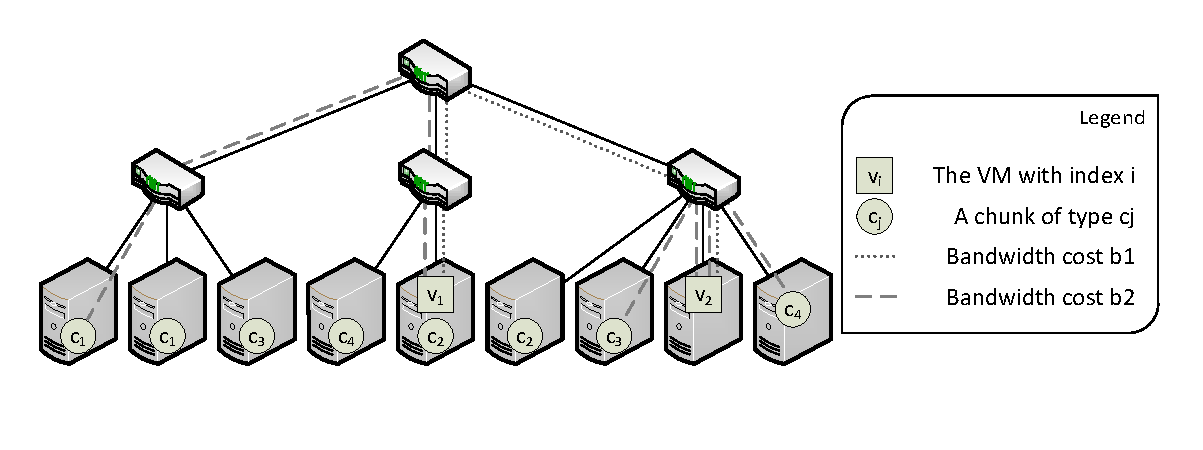
\includegraphics[width=0.99\columnwidth]{figs/overview-fig.pdf}
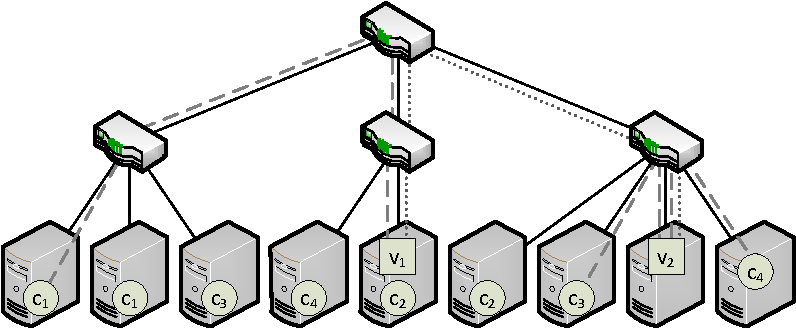
\includegraphics[width=0.79\columnwidth]{figs/data_locality_no_legend.pdf}
\caption{Overview: a 9-server datacenter storing~$\tau=4$ different chunk
types~$\{c_1,\ldots,c_4\}$ (depicted as \emph{circles}). The chunk replicas need to be selected and assigned to the two
 virtual machines~$v_1$ and~$v_2$; the virtual machines are depicted as \emph{squares}, and
 the network connecting them to chunks (at bandwidth~$\CostTrans$) is \emph{dashed}. In addition, the virtual machines are inter-connected among
 each other at bandwidth~$\CostCom$ (\emph{dotted}). The objective of the embedding algorithm is to minimize the overall bandwidth allocation
 (sum of \emph{dashed} and \emph{dotted} lines).}\label{fig:overview}
\vspace{-1em}
\end{figure}


\subsection{Background and Practical Motivation}

Our model is motivated by batch-processing applications such as MapReduce.
Such applications use multiple virtual machines to
process data, often redundantly stored in a distributed file system implemented
by multiple servers.~\cite{local-schedule-1,mapreduce}
The standard datacenter topologies today are (multi-rooted) fat-tree resp.~\emph{Clos} topologies~\cite{fattree,vl2},
hierarchical networks  recursively made of sub-trees at each level;
servers are located at the
tree leaves. Given the amount of multiplexing over the mesh of links
and the availability of multi-path routing protocol, e.g.~ECMP, the redundant
links can be considered as a single aggregate link for bandwidth
reservations~\cite{oktopus,infocom16,ccr15emb,proteus}.

During execution, batch-processing applications typically cycle through different phases,
most prominently, a map phase and a reduce phase; between the two phases,
a shuffling operation is performed, a phase where the results from the mappers
are communicated to the reducers. Since the shuffling phase can constitute a
non-negligible part of the overall runtime~\cite{orchestra},
and since concurrent network transmissions can introduce interference and
performance unpredictability~\cite{amazonbw}, it is important
to provide explicit minimal bandwidth guarantees~\cite{talk-about}.
In particular, we model the virtual network connecting the virtual machines
as a virtual cluster~\cite{oktopus,talk-about,proteus};
however, we extend this model with a notion of data-locality.
In particular, we distinguish between the bandwidth needed between the assigned chunk
and virtual machine ($\CostTrans$) and the bandwidth needed between
two virtual machines ($\CostCom$). 
%Finally, note that it is frequently assumed
%that the nodes implementing the mapper functionality also implement the reducer functionality,
%and vice versa.
% however, it can also make sense to have more mappers or more reducers for
%certain applications.

\subsection{Formal Model}

Let us now introduce our model more formally. 
The model combines three components: (1) the substrate network (the servers
and the connecting physical network),
(2) the input which needs to be processed (divided into data chunks), and
(3) the virtual network (the virtual machines and the logical network connecting the machines to each other
as well as to the chunks).

\textbf{\emph{The Substrate Network.}} The substrate network (also known as the \emph{host graph}) represents the physical resources:
a set~$S$ of~$n_S=|S|$ servers interconnected by a network consisting of a set~$R$ of routers (or switches)
and a set~$E$ of (symmetric) links; we will often refer to the elements in~$S\cup R$
as the \emph{vertices}. We will assume that the inter-connecting network forms an (arbitrary, not necessarily balanced
or regular) tree,
where the servers are located at the tree leaves.
Each server~$s\in S$ can host a certain number
of virtual machines (available server capacity~$\capacity(s)$), and each link~$e\in E$ has a certain bandwidth
capacity~$\capacity(e)$.

\textbf{\emph{The Input Data.}} The to be processed data constitutes the input to the batch-processing application.
The data is stored in a distributed manner; this spatial distribution is given and not subject to optimization.
% Maybe remove the not subject part, due to the comment of reviewer D.
The input data consists of~$\tau$ different \emph{chunk types}~$\{\achunk_1, \ldots, \achunk_{\ChunkType}\}$,
where each chunk type~$\achunk_i$ can have~$r_i\geq 1$ instances (or replicas)~$\{\achunk_{i}^{(1)},\ldots, \achunk_{i}^{(r_i)}\}$,
 stored at different servers. A single server may host multiple chunks.
It is sufficient to process one replica, and we will sometimes refer to this
replica as the \emph{active} (or selected) replica.

\textbf{\emph{The Virtual Network.}} The virtual network consists of a set~$\VirtualNodes$ of~$n_V=|\VirtualNodes|$ virtual machines,
henceforth often simply called \emph{nodes}.
Each node~$v \in \VirtualNodes$ can be placed (or, synonymously, \emph{embedded}) on a server; this placement can be subject
to optimization.

Depending on the available capacity~$\capacity(s)$ of server~$s$, multiple nodes may be hosted on~$s$.
We will denote the server~$s$ hosting node~$v$ by~$\pi(v)=s$.
Since these nodes process the input data, they need to be assigned and connected to the
chunks. Concretely, for each chunk type~$\achunk_i$, exactly one
replica~$\achunk_{i}^{(j)}$ must be processed by exactly one node~$v$;
which replica~$\achunk_{i}^{(k)}$ is chosen is subject to optimization, and
we will denote by~$\mu$ the assignment of nodes to chunks.
%We will typically assume that there are~$\MaFactor\geq 1$ times more chunk types to be processed than there are nodes,
%where~$\MaFactor$ is an integer;
%We will keep the model general, and consider both the case where there are more chunk types
%than virtual machines (requiring the assignment of multiple chunks per nodes) and the case
%where there are less chunks than virtual machines. (See below for motivations for the different scenarios.)
%each node needs to process the same number of chunks.

In order to ensure a predictable application performance, both the connection to the chunks
as well as the interconnection between the nodes may have to ensure certain
minimal bandwidth guarantees; we will refer to the first type of virtual network as the \emph{(chunk) access
network}, and to the second type of virtual network as the \emph{(node) inter-connect}; the latter
is modeled as a complete network (a \emph{clique}). Concretely, we assume that an  active chunk
is connected to its node at a minimal (guaranteed) bandwidth~$\CostTrans$, and a node is connected to any other node
at minimal (guaranteed) bandwidth~$\CostCom$.

%Note that we do not explicitly model the process of
%copying back the final results from the
%reducers to the file system: this step offers many flexibilities,
%and can be done based on the current network state~\cite{endpoint}; it does not require
%explicit reservations.

%\stefan{TODO: clarify whether there can be multiple chunks and or nodes per server}

%\textbf{Optimization Objective.}

\subsection{Optimization Objective}

Our goal is to develop algorithms which 
accept and embed a request
whenever this is possible, and minimize the \emph{resource footprint}: the amount of resources which have to be dedicated to a request, in order to realize its guarantees.
%Our goal is to develop algorithms which minimize
%the \emph{resource footprint}: the guaranteed bandwidth allocation (or synonymously: %\emph{reservation}) on all links of the given embedding; note that
%only the resource allocation at the links but not at the servers depends on the replica selection or %embedding. Thus,
%we on the one hand aim to embed the nodes in a locality-aware manner, close to the input data
%(the chunks), but at the same time also aim to embed the nodes as close as possible to
%each other.

Formally, let~$\dist(v,\achunk)$ denote the distance (in the underlying physical network~$\Tree$) between a node~$v$ and
its assigned (active) chunk replica~$\achunk$, and let~$\dist(v_1,v_2)$ denote the distance between the two nodes~$v_1$ and~$v_2$.
We define the \emph{footprint}~$\Cost(v)$ of a node~$v$ as follows:
$$
\Cost(v) = \sum_{\achunk\in \mu(v)} \CostTrans \cdot \dist(v,\achunk) \underbrace{+ \frac{1}{2} \cdot \sum_{v' \in \VirtualNodes\setminus\{v\}} \CostCom \cdot \dist(v,v')}_{\text{only for inter-connect}},
$$
 where~$\mu(v)$ is the set of chunks assigned to~$v$. Our goal is to minimize the overall footprint
$\Cost=\sum_{v\in V} \Cost(v)$.
% Recall Figure~\ref{fig:overview}.

%\textbf{Problem Decomposition.}

\subsection{Problem Decomposition}

In order to chart the landscape of the computational tractability and intractability of different
problem variants, we decompose our problem into its fundamental aspects, namely replica selection
($\RS$), multiple chunk assignment ($\MA$), flexible node placement ($\FP$), node interconnect ($\CC$),
and bandwidth constraints ($\BW$), as described in the following. 
In this paper, we will consider all possible 32 problem variants, where each of these five aspects
can either be enabled or disabled. 

\textbf{\emph{Replica Selection ($\RS$).}} The first fundamental problem is replica selection:
if the input data is stored redundantly, the algorithm has the freedom to choose a replica
for each chunk type, and assign it to a virtual machine (i.e., \emph{node}).
In the following, we will refer to a scenario
with redundant chunks by~$\RS$; in the~$\RS$-only scenario, the number of chunk types
is equal to the number of nodes. Otherwise, we will add the~$+\MA$ property discussed next.

\textbf{\emph{Multiple Assignment ($\MA$).}}
If the number of chunk types~$\tau$ is larger than the number of nodes,
each node needs to be assigned multiple chunks. We will refer to such a scenario by~$\MA$. 
Since all nodes are identical and no additional information regarding the chunks is available at request time, we assume that each node will process an identical integer number of chunks~$\MaFactor = \tau / n_V$. 
%We will refer to such a scenario by~$\MA$,
%and will denote the number of chunks per node by the integer value~$\MaFactor = \tau / n_V$ (a constant).


\textbf{\emph{Flexible Placement ($\FP$).}} %The third fundamental degree of freedom, besides replica selection and assignment,
%regards the flexibility in the placement (or synonymously: \emph{embedding}) of nodes on physical servers.
%We will refer to this aspect by~$\FP$.
While the nodes are placed a priori in some cases, the node placement (or
synonymously: \emph{embedding}) of nodes on physical servers can also be
subject to optimization. We will refer to this degree of freedom by FP.
%(Recall that each server~$s$ can host~$\capa(s)$ nodes.)

\textbf{\emph{Node Interconnect ($\CC$).}} We distinguish between scenarios
where bandwidth needs to be reserved
both from each node to its assigned chunks as well as to the other nodes
(i.e.,~$\CostTrans>0$ and~$\CostCom>0$), and
 scenarios where only the (chunk) access network requires bandwidth reservation (i.e.,~$\CostTrans>0$ and~$\CostCom=0$).
 We will refer to the former scenario
where bandwidth needs to be reserved also for the inter-connect, by~$\CC$. 
The node interconnect is modelled as a complete graph, to account for the all to all communication patterns of batch processing applications such as MapReduce.

%We also note that the case~$\CostTrans=0$ and~$\CostCom>0$ has been studied in prior %work~\cite{oktopus,talk-about,proteus},
%and refer the reader to our related work section.


\textbf{\emph{Bandwidth Capacities ($\BW$).}}
We distinguish between an uncapacitated and a capacitated scenario where the links
of the substrate network come with bandwidth
constraints, and will refer to the bandwidth-constrained version by~$\BW$; the capacity of servers
(the number of nodes which can be hosted concurrently) is always limited.
Note that capacity constraints introduce infeasible problem instances, where it is impossible to
allocate sufficient resources to satisfy an embedding request.

%\textbf{Remark on Practical Motivation.}

%%%%%%%%%%%%%%%%%%%%%%%%%%%%%%%%%%%%%
\section{Polynomial-Time Algorithms}\label{sec:poly}


Despite the various degrees of freedom in terms of embedding and replica selection,
we can solve many problem variants efficiently.
 This section introduces three general techniques,
 which can roughly be categorized into
 \emph{flow} (Section~\ref{ssec:flow}), \emph{matching} (Section~\ref{ssec:match}) and \emph{dynamic programming}
 (Section~\ref{ssec:dyn}) approaches.
% As we will see, sometimes multiple approaches can be used to solve a given problem variant, %however,
 %runtimes can differ.
%For each approach, we will summarize the solvable problem variants using a \emph{Venn diagram}.
First, let us make a simplifying observation:
\begin{obs}\label{obs:nofp}
In problems without flexible placement ($\FP$),
the bandwidth required
for the inter-connect network ($\CC$) can be allocated \emph{upfront}, 
as it
does not depend on the replica
selection and assignment.
Accordingly, we can reduce problem variant~$\RS+\MA+\CC +\BW$ (as well as all its subproblems)
to~$\RS+\MA+\BW$ (resp.~its subproblems).
\end{obs}

\subsection{Flow Algorithms ($\RS+\MA+\CC+\BW$)}\label{ssec:flow}


\begin{figure}[t]
\centering
%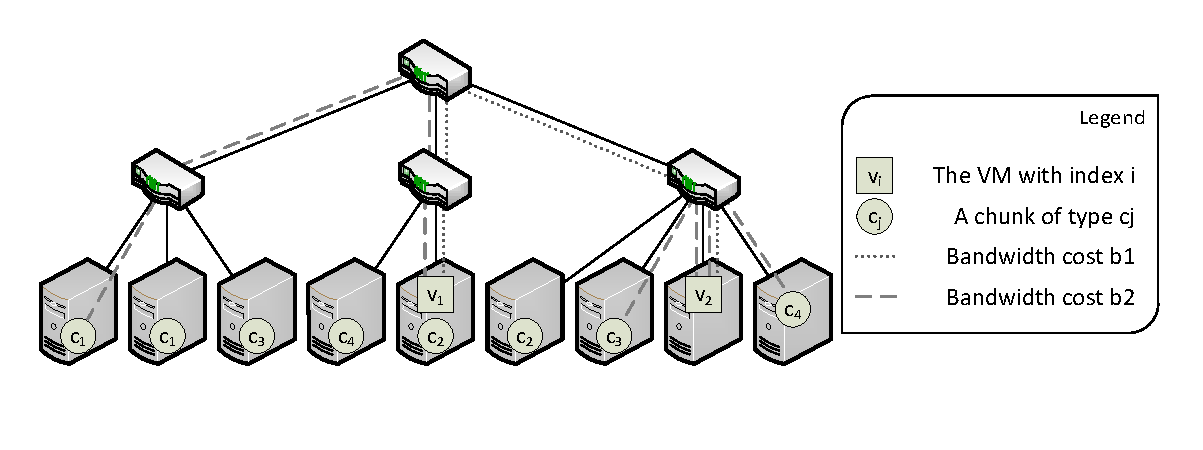
\includegraphics[width=0.99\columnwidth]{figs/overview-fig.pdf}
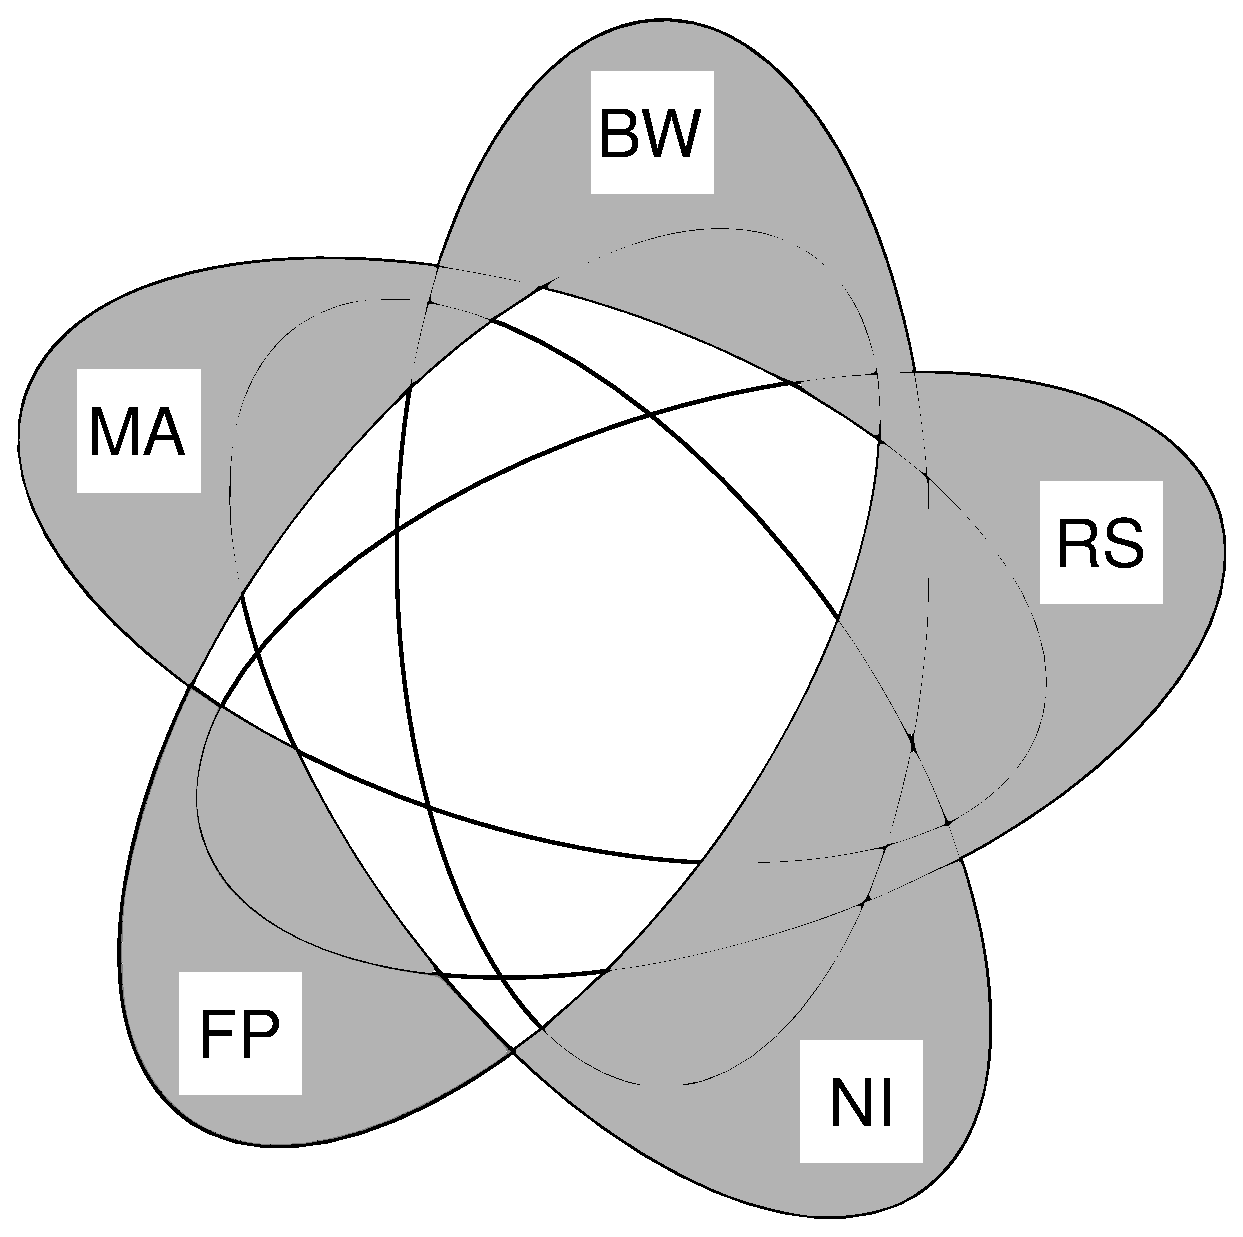
\includegraphics[width=0.49\columnwidth]{figs/venn_flow.pdf}
\caption{Variants solved by flow approach.}
\vspace{-1em}
\label{fig:venn_flow}
\end{figure}


We first present an algorithm to solve the~$\RS+\MA+\CC+\BW$ problem.
Recall that in this problem variant,
we are given a set of redundant chunks ($\RS$) and a set of
nodes
(the \emph{nodes})
at fixed locations (no~$\FP$). The number of chunk types is larger than the number
of nodes ($\MA$), and each node needs to be connected
to its selected chunks as well as to other nodes ($\CC$), while respecting
capacity constraints ($\BW$).
Our goal is to minimize the resource footprint~$\Cost$, consisting
of the bandwidth reservations in the (chunk) access network and the (node)
inter-connect.
As we will see in the following, we can use a flow approach to solve this
problem variant.



%We allow an instance to have multiple nodes in single leaf.

\textbf{Construction of Artificial Graph.}
In order to solve the~$\RS+\MA+\CC+\BW$ problem,
we first remove the~$\CC$ property using Observation~\ref{obs:nofp}.
We then construct
an artificial graph~$\Tree^*$, extending the substrate network~$\Tree$ and
normalizing bandwidth capacities, as follows. For~$\Tree^*$,
we normalize the bandwidth of~$\Tree$ to integer multiples of~$\CostTrans$,
i.e., for each link~$e\in E(\Tree)$, we set its new
capacity in~$\Tree^*$ to~$\lfloor\capacity(e)/\CostTrans\rfloor$.
After this normalization, we extend the topology~$\Tree$ by
introducing an artificial vertex for each chunk type. These artificial
vertices are connected to each leaf (i.e., server) in~$\Tree$ where a replica
 of the respective chunk type is located,
connecting the replica of the respective chunk type by a link of capacity~$1$. In
addition, we create a
\emph{super-source}~$\Source$, and connect it to each of the artificial chunk
type vertices (with a link of capacity 1). Moreover, we create an artificial \emph{super-sink}~$\Sink$ and
connect it to every leaf containing at least one node; the link capacity represents
the number of nodes~$x$ hosted on this server, times the multi-assignment factor
$\MaFactor$.
We additionally assign the following costs to edges of~$\Tree^*$:
every edge of the original substrate network costs one unit, and all other artificial edges
cost nothing.

%Recall that~$\RS+\CC+\MA+\BW$ boils down to
%$\RS+\MA+\BW$ in the absence of~$\FP$
A solution to the~$\RS+\MA+\BW$ problem can now be computed
from a solution to the \emph{Min-Cost-Max-Flow} problem between super-source
$\Source$ and
super-sink~$\Sink$ on the artificial graph~$\Tree^*$.

\textbf{Example.} Figure~\ref{fig:flow_construction} shows an example of the extended substrate
network~$\Tree^*$: The sink~$\Sink$ is connected to the two leaves, which host the
nodes. The artificial nodes are depicted below the leaves, are labeled with
their respective chunk types (e.g.,~$\achunk_1$), and are connected to the source
$\Source$ as well as to the leaves which contain replicas of their chunk type.
The
maximum flow with minimal costs is indicated by the dashed lines: each line
represents one unit of flow. The dotted lines indicate links which have reduced
capacity due to~$\CC$.

\begin{figure}
\centering
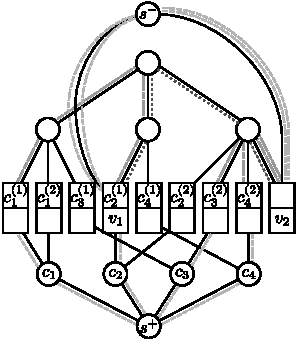
\includegraphics[width=0.45\columnwidth]{figs/flow_ma_cv}
\caption{Example of flow construction: Problem instance with two nodes, four chunk
types, and two replicas per type. The min-cost-max-flow
is indicated by the dashed lines: each line represents one unit of flow.
}
\vspace{-1em}
\label{fig:flow_construction}
\end{figure}

\textbf{Algorithm.}
Our algorithm to solve~$\RS+\MA+\CC+\BW$ consists of three parts:
\emph{First}, we construct the normalized and extended graph~$\Tree^*$
described above and compute
a min-cost-max-flow solution, e.g.,
using~\cite{mincostmaxflow-1,mincostmaxflow-2}.
\emph{Second}, we have to \emph{round} the resulting, possibly fractional flow, to
integer values. Due to the \emph{integrality theorem}~\cite{flow-book},
there always exists an optimal integer solution on graphs with integer capacities.
However, while algorithms like the successive shortest path algorithm~\cite{successive_shortest_path_complexity}
directly give us such an integral solution (in polynomial time), the fastest min-cost-max-flow algorithms (e.g., based on double-scaling
methods~\cite{mincostmaxflow-1} or minimum mean-cost cycle
algorithms~\cite{mincostmaxflow-2}, may yield fractional solutions
which need to be rounded to integral solutions (of the same cost).
In order to compute integral solutions, we proceed as follows: we iteratively
pick an arbitrary (loop-free) path
currently having a fractional allocation of value~$f$ ($f>0$), and distribute its flow~$f$
among all other fractional paths of the same length; due to the optimality of the fractional solution
and due to the integrality theorem, such paths must always exist. After distributing this flow,
the total allocation on this path will be 0, and we have increased the number of
integer paths by at least one. We proceed until we constructed the perfect
matching.
\emph{Third}, given an integer min-cost-max-flow solution, we need to decompose
the integer flow into the paths
representing matched chunk-node pairs:
The assignment can be obtained by decomposing the flow allocated in the
original substrate network. In order to identify a matched chunk-node pair,
we take an arbitrary (loop-free) path~$p$ carrying a flow of value ~$\geq 1$ from~$\Source$ to~$\Sink$:
the first hop represents the chosen chunk type, the second hop the chosen
replica, and the last but one hop represents the server: we will assign
the replica to an arbitrary unused node on this server.
Having found this pair, we reduce the flow
along the path~$p$ by one unit.
We continue the pairing process until every chunk type is assigned.

\textbf{Analysis.}
The correctness of our approach follows from our construction
of~$\Tree^*$, using integer capacities (in our case~$\lfloor\capacity(e)/\CostTrans\rfloor$),
and the fact that cost optimal integral solutions always exist~\cite{flow-book}.
The runtime of our algorithm consists of four parts: construction of~$\Tree^*$,
computation of the min-cost-max-flow, flow rounding, and decomposition. The
dominant term in the asymptotic runtime is the flow computation.
Using the state-of-the-art min-cost-max-flow
algorithms~\cite{mincostmaxflow-1,mincostmaxflow-2}
we get a runtime of~$\mathcal{O}(n_S^2 \cdot \log\log \min \{U,\tau\})$
where~$U$ is the maximal link capacity; note that in networks with high capacity
and uncapacitated networks, we can simply set~$U=\tau$.
% resp.~$\mathrm{O}(n_S^5 \cdot \tau^3 \log n_S)$, where~$\delta$ is the network diameter and
%where~$U$ is the maximal link capacity in the substrate;
%using~\cite{successive_shortest_path_complexity},
%together with the Dijkstra shortest-path algorithm we have~$\mathrm{O}(n_S^2\cdot \tau)$.

%\textbf{Summary.}
%Figure~\ref{fig:venn_flow} summarizes all problem
%variants which can be solved with our flow-based approach.

\subsection{Matching Algorithms ($\RS+\MA+\CC$ and~$\MA+\CC+\BW$)}\label{ssec:match}


\begin{figure}[t]
\centering
%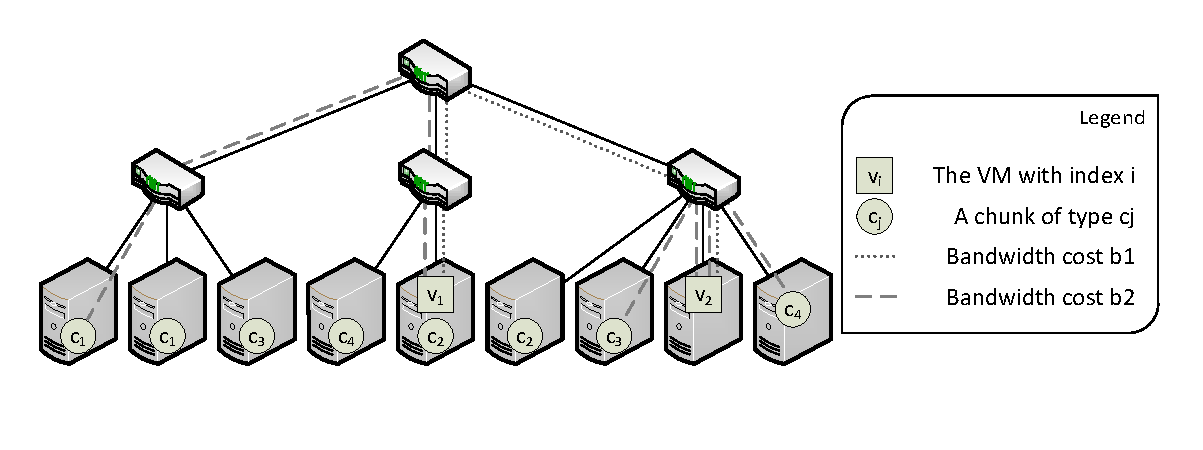
\includegraphics[width=0.99\columnwidth]{figs/overview-fig.pdf}
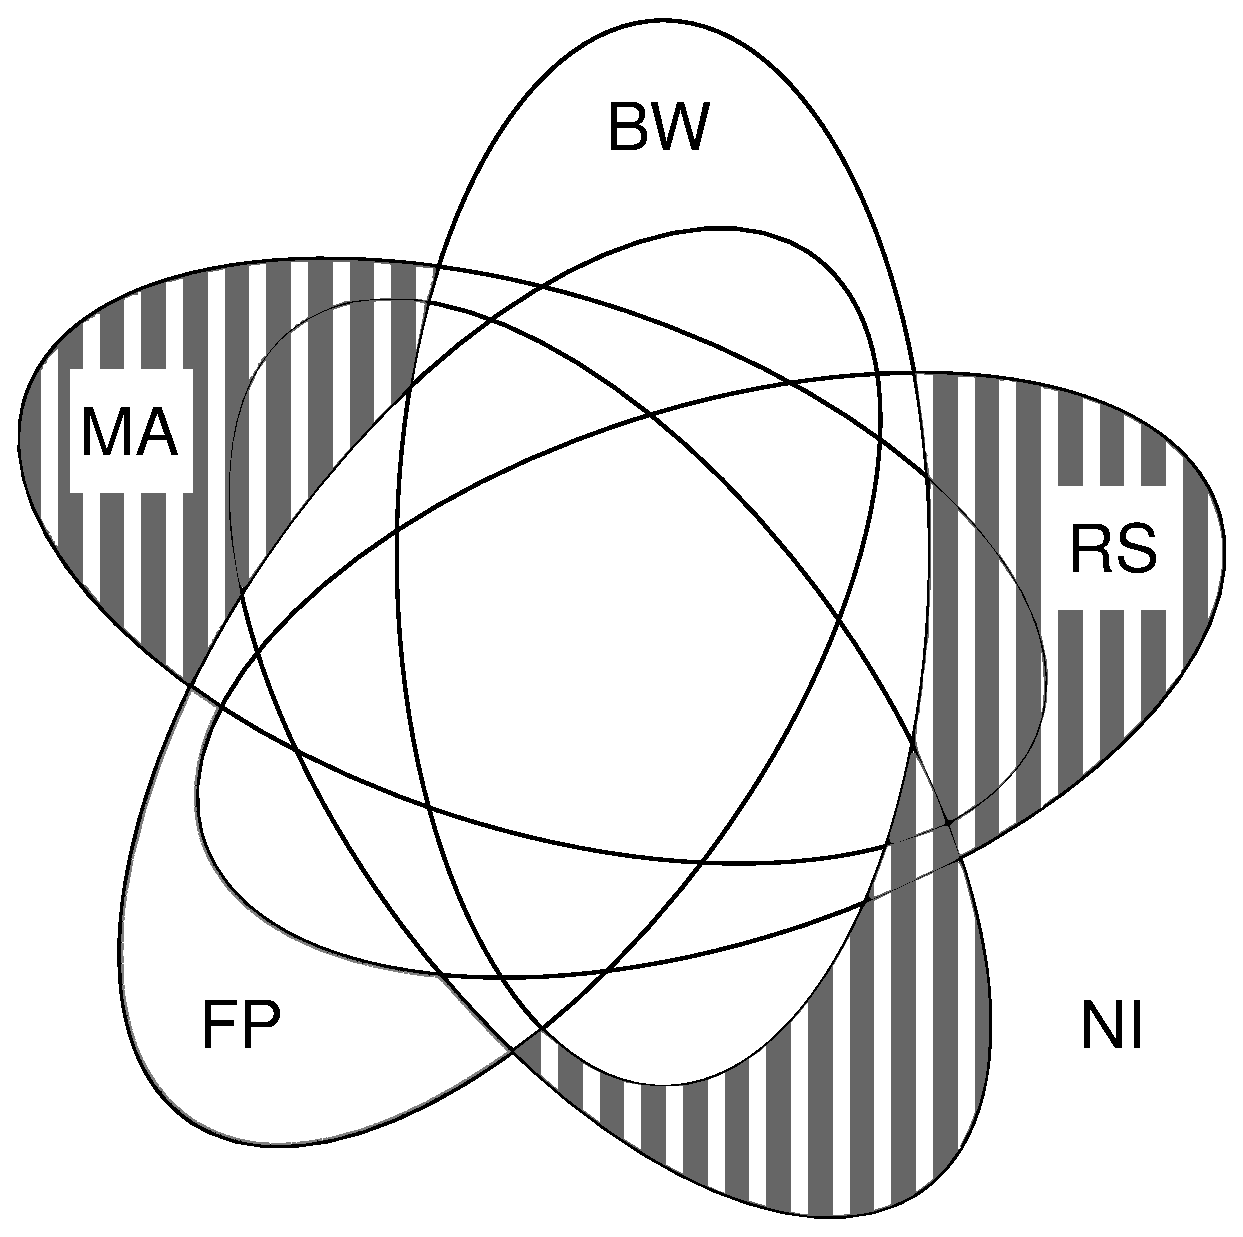
\includegraphics[width=0.49\columnwidth]{figs/venn_matching.pdf}
\caption{Variants solved by matching approaches.}
\vspace{-1em}
\label{fig:venn_match}
\end{figure}
This section presents faster algorithms to solve 
the two problem variants
$\RS+\MA+\CC$ and~$\MA+\CC+\BW$ which can also be solved with the flow approach
introduced above.
In general, we refer to the algorithms presented in this section
as matching approaches.


\subsubsection{$\RS+\MA+\CC$}

Let us first consider the~$\RS+\MA+\CC$ variant.
Recall that in this problem,
we are given a set of redundant chunks ($\RS$) and a set of nodes
at fixed locations. The number of chunk types is larger than the number
of nodes ($\MA$), and each node needs to be connected
to its chunks as well as to other nodes ($\CC$).
Our goal is to minimize the resource footprint~$\Cost$, consisting
of the bandwidth reservations in the access network and the inter-connect.

\textbf{Algorithm.} Due to Observation~\ref{obs:nofp},~$\RS+\MA+\CC$ degenerates to~$\RS+\MA$.
In order to solve the~$\RS+\MA$ problem variant,
we construct a bipartite
graph between the set
$\VirtualNodes$ of nodes and
the set of chunks.
Concretely, we clone each node~$\MaFactor$ times,
as each node needs to process
$\MaFactor$ chunk types, and we collect all copies of a given chunk type in a
single %$\ChunkType$
``super-node''. We connect each node to all chunk types using the
\emph{lowest hop count} to one of the copies as the cost metric (the link weight).
On the resulting bipartite graph, we can now compute a \emph{Minimum Weight
Perfect
Matching}~\cite{gabow_scaling_algorithm}:
the resulting matching describes the optimal assignment of chunks to nodes.

%\begin{figure}[h]
%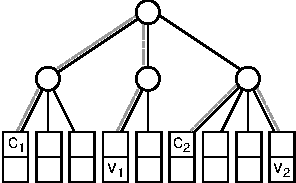
\includegraphics[width = 0.49\columnwidth]{figs/matching_topology_simple}
%\hfill
%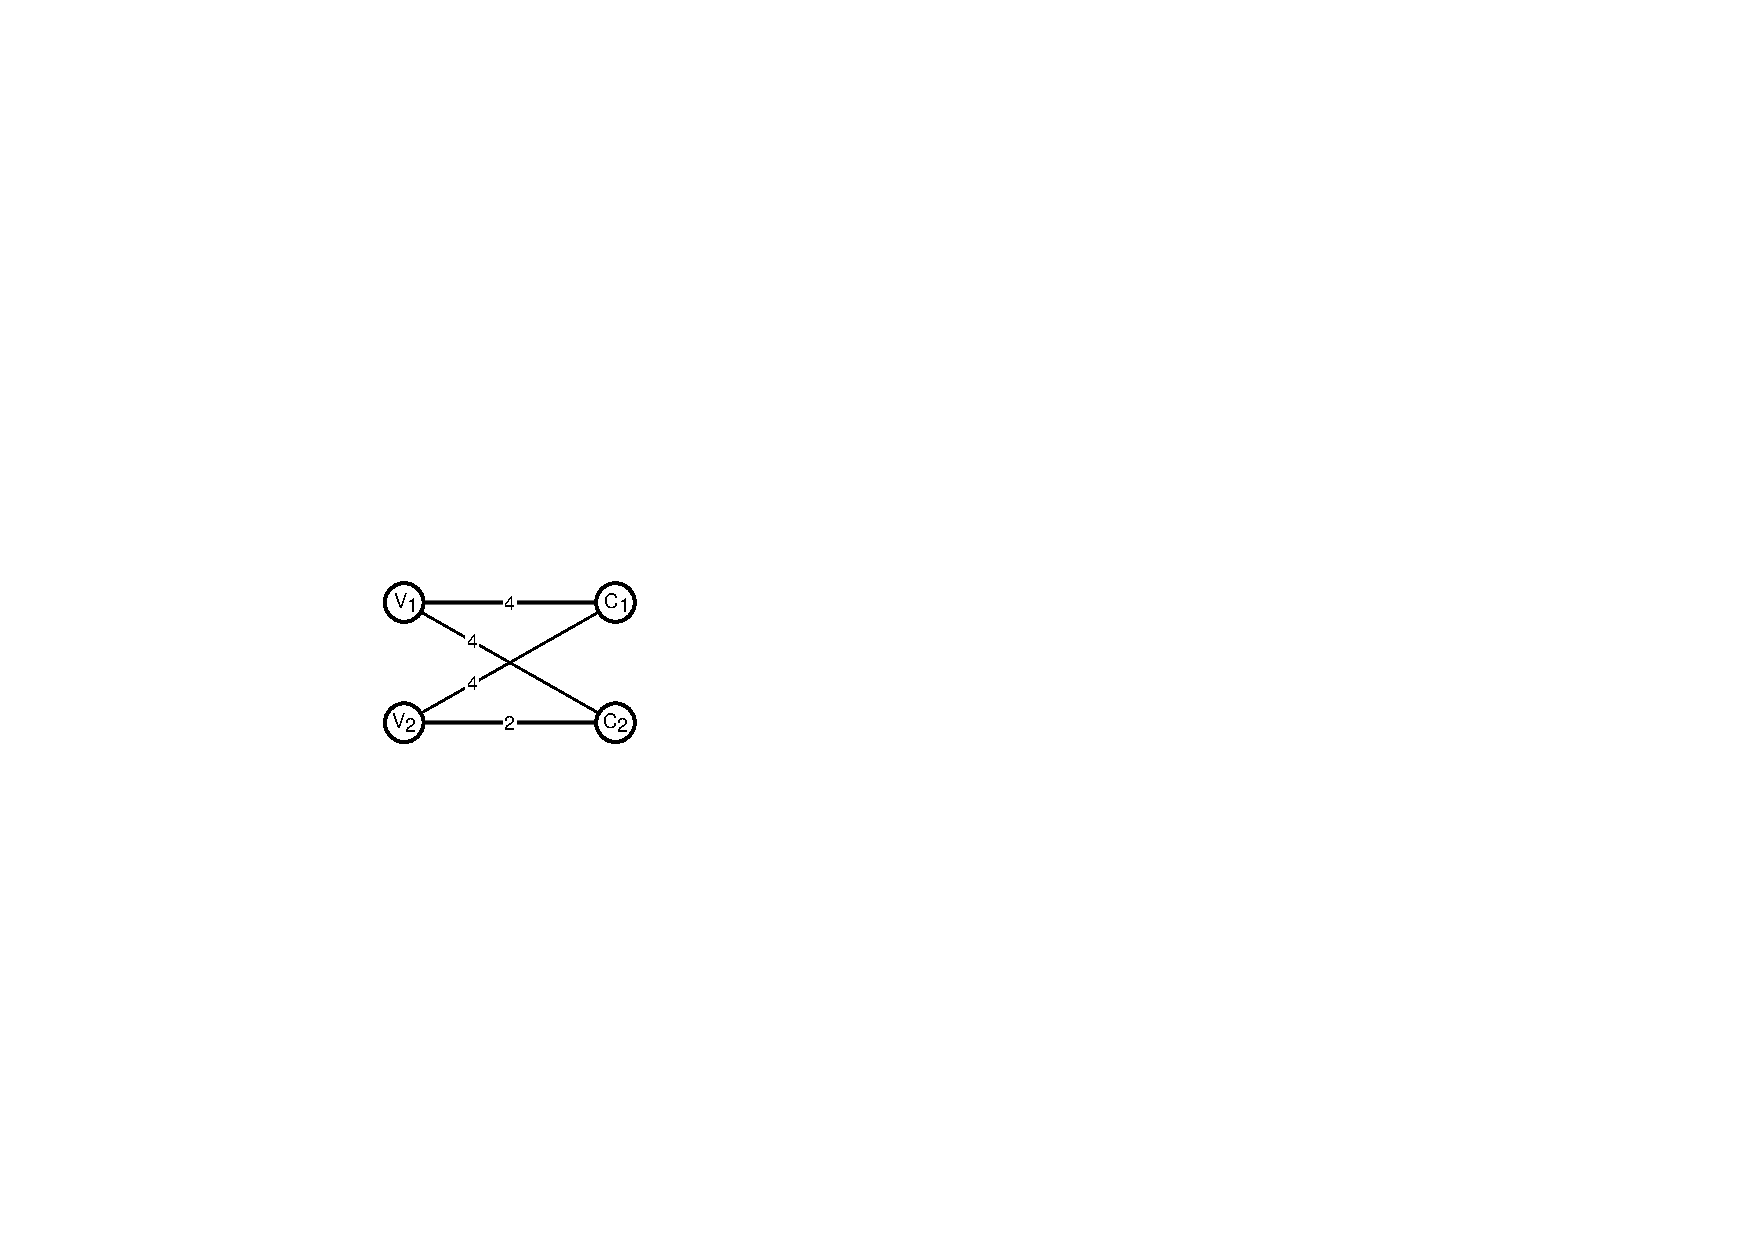
\includegraphics[width =0.4\columnwidth]{figs/matching_basic}
%\caption{The problem instance on the \emph{left} consists of
%two nodes and two chunks. The
%optimal solution is indicated by the dashed lines. The corresponding matching
%problem on the \emph{right} represents the same situation. The weights on the
%edges
%are set according to the distance in the substrate. The solution of the minimum
%cost perfect matching is depicted by the shaded lines.}
%\label{fig:matching_basic}
%\end{figure}

\begin{figure}
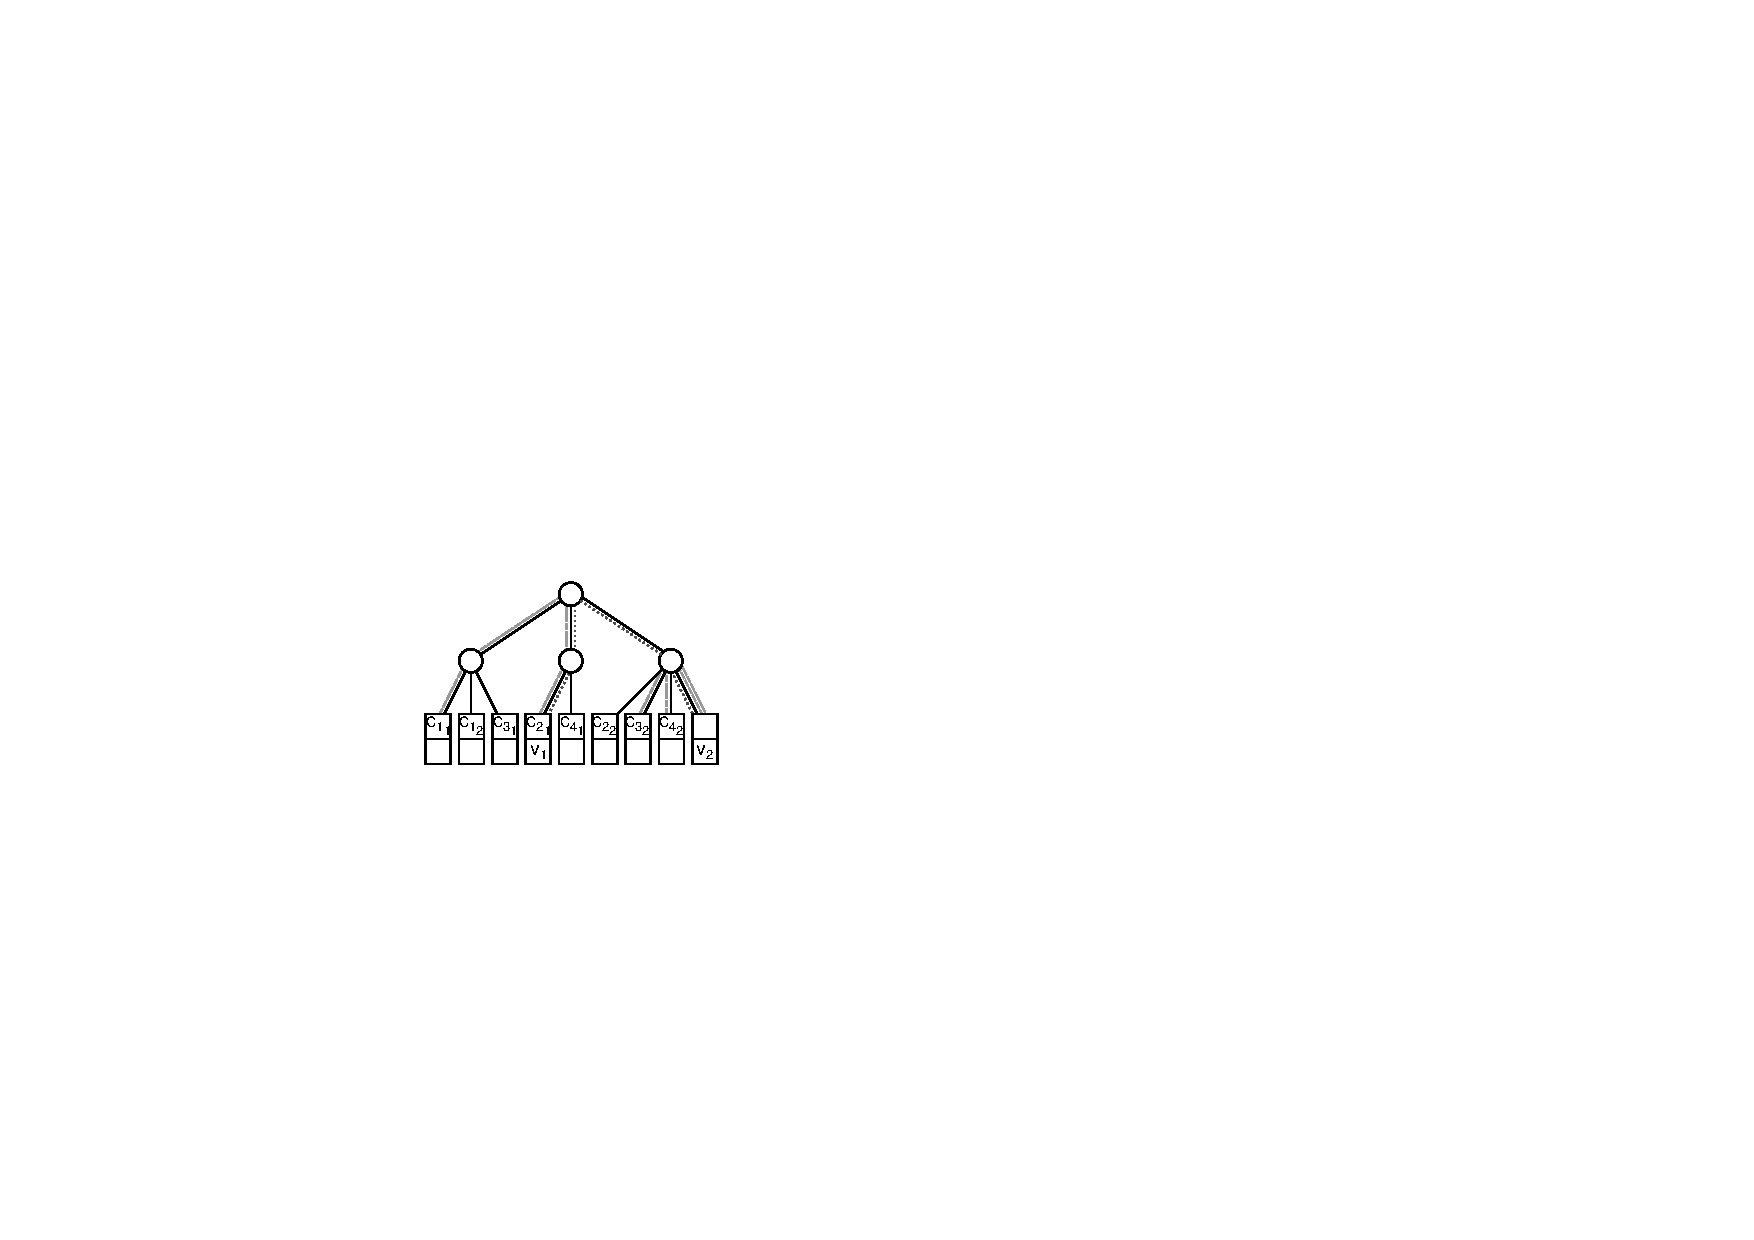
\includegraphics[width = 0.49\columnwidth]{figs/model_ma_r_cv_boxes}
\hfill
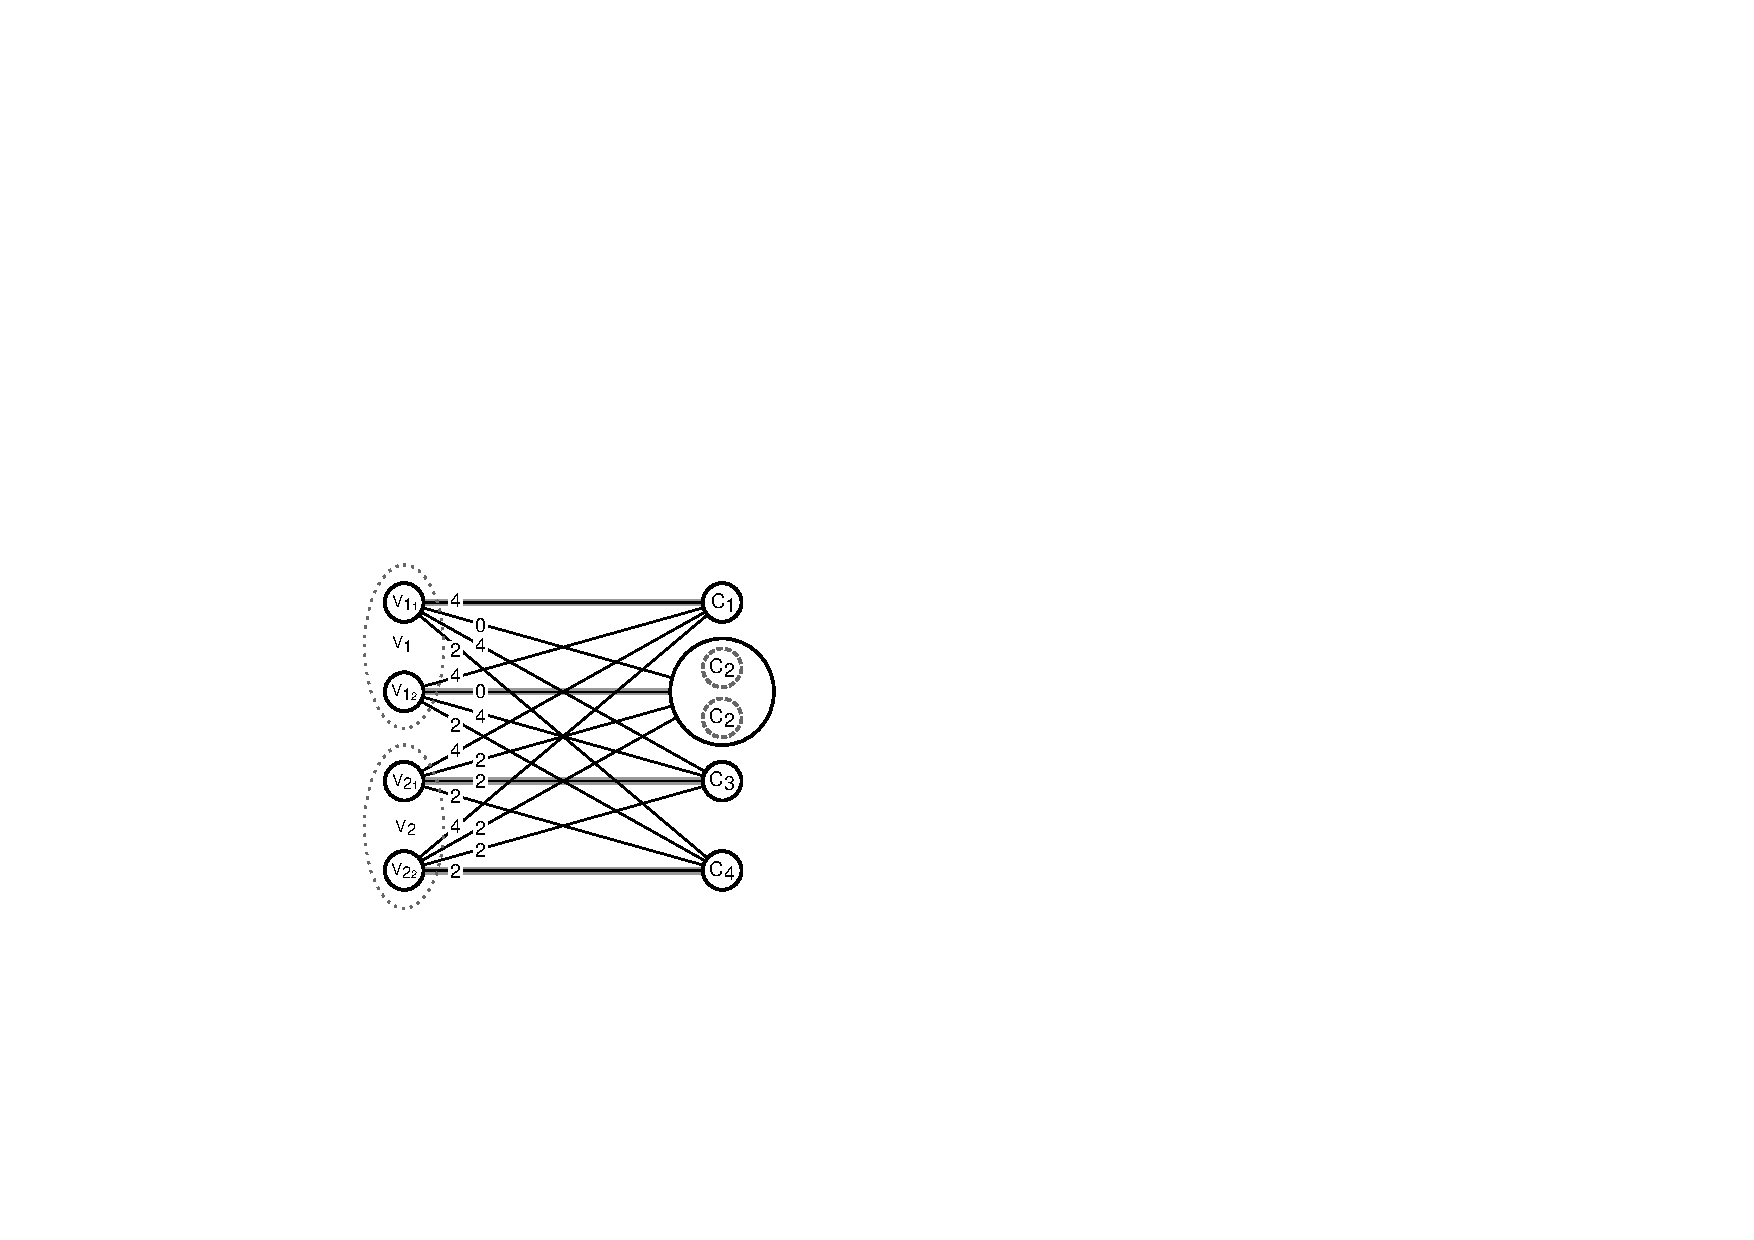
\includegraphics[width =0.49\columnwidth]{figs/matching}
\caption{The~$\RS+\MA$ problem on the \emph{left} is converted into a
matching problem on the \emph{right}. Since each node has to process two
chunks, the
nodes are replicated in the matching representation. The two replicas of each
chunk type are represented by a single node, and all edges connecting to this
node have a weight according to the shorter distance to one of the replicas.
This is visualized for~$\achunk_2$.}
\label{fig:matching}
\end{figure}

\textbf{Example.} Before analyzing our algorithm, let us consider a small example.
Figure~\ref{fig:matching} illustrates
an instance where two nodes are
cloned into~$\MaFactor = 2$ nodes each,
resulting in a total of four nodes in
the matching problem representation.
The two replicas of each chunk type are
aggregated into a single chunk type vertex~$\achunk_j$  in the matching problem;
this gives a total of four chunk type vertices in the matching graph. The costs
on the links between all clones of a specific vertex and a chunk type are set to
the minimum distance. We can observe this for instance at the edges connecting
the two clones of~$\VirtualNode_1$ to~$\achunk_2$: both weights are 0.

\textbf{Analysis.}
The correctness of our algorithm follows from the construction and the optimal
solution of the minimum matching.
The runtime consists of two parts: the construction of the matching graph and
the actual matching computation. The constructed graph consists of
$\MaFactor \cdot n_V \cdot \ChunkType$
many edges,
and for each edge we need to compute its cost, i.e., the shortest distance
which in a tree can be computed in time~$n_S$; thus, the overall construction time
is
$\mathcal{O}(n_S \cdot \tau^2)$.
The state of the art algorithm to compute matchings are based on scaling techniques~\cite{scale-match}.
The runtime translates to
$\mathcal{O}(\tau^{5/2}\cdot \log(\tau\cdot n_S))$; recall that~$\tau = \MaFactor\cdot n_V$.




\subsubsection{Faster~$\MA+\CC$ and~$\MA+\CC+\BW$}

We now show that we can solve~$\MA+\CC$ even faster, by exploiting
locality. Moreover, we will show that we can
even solve
$\MA+\CC+\BW$ problem variants by simply
verifying feasibility.
In the following, due to Observation~\ref{obs:nofp}, we can focus on
the~$\MA$ resp.~$\MA+\BW$ problem.

We first introduce the following definition.
\begin{defn}[Local Assignment (LA)]\label{def:loc}
We define an assignment~$\VmChunkAssignment$ to
be \emph{local in a specific subtree~$\Tree'$}, iff~$\VmChunkAssignment$
assigns the maximum number of chunks in the
subtree to nodes in the same subtree.
% (subject only to the number of available nodes
%in~$\Tree'$).
We define~$\VmChunkAssignment$ to be \emph{local} when
it is local with respect to all possible subtrees of the substrate network.
\end{defn}

\begin{figure}
\center
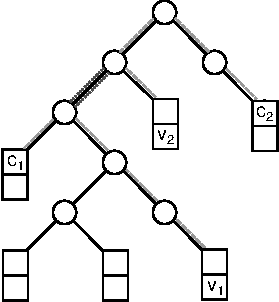
\includegraphics[width = 0.45\columnwidth]{figs/unbalanced_tree}
\caption{Illustration of local assignment: The dashed lines indicate bandwidth allocations, which occur
independently of the chosen assignment. The dotted lines indicate bandwidth
allocation which occur only if~$c_2$ is assigned to~$v_1$.}
\label{fig:unbalanced_tree}
\end{figure}

\textbf{Example.}
Figure \ref{fig:unbalanced_tree} illustrates the concept of local assignment:
The closest chunk to~$v_2$ is~$c_1$, and the closest node to~$c_1$ is~$v_2$.
However, a subtree~$T'$ exists such that~$v_1 \in T'$ and~$c_1
\in T'$, but~$v_2 \notin T'$. Therefore, a local assignment cannot assign~$c_1$ to~$v_2$.

% shows an instance with two chunks and
%two nodes. A local assignment assigns~$v_1$ to~$c_1$, although~$c_2$ is
%closer to~$v_1$, since a subtree~$T'$ exists,


We will see later that
optimal solutions to
$\MA$ have a local assignment. We exploit this in our algorithms described
in the following.

\textbf{Algorithm.} Our proposed algorithm for~$\MA$
proceeds in a bottom-up fashion, traversing the substrate network~$\Tree$
from the leaves toward the root.
For each subtree~$\Tree'$, we maintain
two sets~$S_1,S_2$ in order to match unmatched
chunks~$S_1$ in the subtree~$\Tree'$ to unmatched
nodes~$S_2$ in~$\Tree'$. Both sets are initially empty.

We first process all the leaves, in an arbitrary order; subsequently, we process arbitrary inner vertices
of~$\Tree$, whenever all their children have been processed.
We process any leaf~$\ell$
by adding any
nodes or chunks which are located on~$\ell$ to the corresponding sets~$S_1$ and~$S_2$.
A non-leaf vertex~$u$ is processed in the following way: we take the union of
the sets of~$u$'s children, i.e., the sets contain the unmatched chunks and nodes
in this subtree.
For both leaves and inner nodes, whenever
both sets are non-empty, we greedily match an arbitrary chunk in~$S_1$ with an arbitrary node in~$S_2$,
and remove them from the sets.

\textbf{Analysis.} On a given vertex~$u$, emptying one of the sets, results in a \emph{local assignment} (cf~Definition~\ref{def:loc})
in the
subtree rooted at~$u$. The bottom-up strategy ensures that this works
for every subtree in the substrate, rendering the resulting assignment
local.
The complexity of this
construction is low: For each
vertex in the substrate graph,
we build the union of the
children's sets,
and since each vertex can only be the child of one vertex,
the amortized runtime per vertex is constant; and hence the overall
runtime~$\mathcal{O}(n_S)$. The sum of all remove operations, is equal to
the number of chunk types~$\mathcal{O}(\ChunkType)$.
Hence the overall complexity of this construction amounts to
$\mathcal{O}(n_S + \ChunkType)$.

It remains to prove optimality of such local assignments.
We first characterize the bandwidth allocation on uplinks of subtrees.
\begin{lemma}\label{lem:uplink-alloc}
Given an~$\MA$ problem and a subtree~$\Tree'$
containing~$x$
chunks and~$y$ nodes, the minimal bandwidth allocation of any
assignment
$\VmChunkAssignment$ on the uplink of~$\Tree'$ is~$|x-y\cdot\MaFactor|\cdot
\CostTrans$.
\label{lemma:uplink}
\end{lemma}
\begin{proof}
In case the number of chunk types equals the processing capacities of the
nodes in the given subtree,
the bandwidth allocation inflicted by the chunk access network on the uplink can
be
zero, since we can assign all chunks to nodes in the same subtree.
Otherwise, we distinguish between two cases: Recall, that in instances
without~$\RS$, all chunks have to be processed. In case
there are more chunks in the subtree, at least all of the excess chunks have to
be transferred to a different subtree, which will
inflict costs~$\CostTrans$ per excess chunk on the uplink connecting~$\Tree'$
with the
remaining parts of~$\Tree$, which will inflict costs~$\CostTrans$ per excess chunk on the uplink of root of~$\Tree'$.
 Similarly, if the processing capabilities exceed the
amount of
available chunks, excess chunks from other subtrees will have to be transferred
to
nodes in the subtree~$\Tree'$, inflicting bandwidth costs of~$\CostTrans$ each.
Hence, the minimum bandwidth allocation for the chunk access on the uplink
is the difference between the number of chunks and the processing capabilities
of the subtree~$|x-y\cdot\MaFactor|$ times the amount of bandwidth needed,
for a single transfer~$\CostTrans$.
\end{proof}


\begin{theorem}
Given an~$\MA+\CC$ problem instance, a feasible assignment~$\VmChunkAssignment$
is optimal iff it is local.
\label{thm:local_optimal}
\end{theorem}

\begin{proof}
Local assignments generate exactly the minimal allocations on all links, as
 the assignments which generate the minimal bandwidth allocations
described in
the proof of
Lemma~\ref{lemma:uplink} are local in the given subtree. Hence
each local assignment has to be optimal. A non-local assignment, has at least
one subtree, in which it is not local. This subtree will have a higher
allocation on the uplink. Since the local assignment has minimal allocations
on all other links, the non local assignment has a larger footprint.
\end{proof}



Combined with a simple postprocessing step, this approach can also solve~$\MA+\BW$. The central idea of this extension, is
that \emph{local} assignments allocate the minimal bandwidth
on each individual edge. In consequence, each bandwidth constraint
which is lower than the allocation of a local assignment on one link, renders
the problem infeasible. Hence, it is sufficient to temporarily omit the
bandwidth limitations, compute an optimal assignment for an~$\MA$ instance, and
verify that the resulting allocations do not violate any capacities. The
postprocessing step scales linearly with the number of edges in the substrate
graph.



\subsection{Dynamic Programming ($\MA+\FP+\CC+\BW$)}\label{ssec:dyn}

We now show how to solve the~$\MA+\FP+\CC+\BW$ problem variant
in polynomial time.
Note that this problem variant requires to find a
tradeoff between the desire to place nodes as close as possible to each other
(in order to minimize communication costs), and the desire to place nodes
as close as possible to
the chunk locations.




\textbf{Example.} Figure~\ref{fig:dynamic_motivation} shows an example: one
extreme solution is to minimize the distance between chunks and nodes,
see mapping~$\NodeMapping_1$ in
Figure~\ref{fig:dynamic_motivation} \emph{(left)}: the four nodes are all
collocated with chunks, resulting in a zero-cost chunk access network. As a
result, the paths between the individual nodes are longer than in alternative
node placements: each node has a distance of two hops to one other node,
and four hops to two other nodes. Hence the resulting allocations for the
node interconnect sum up to~$20 \cdot \CostCom$.

\begin{figure}[t]
\centering
%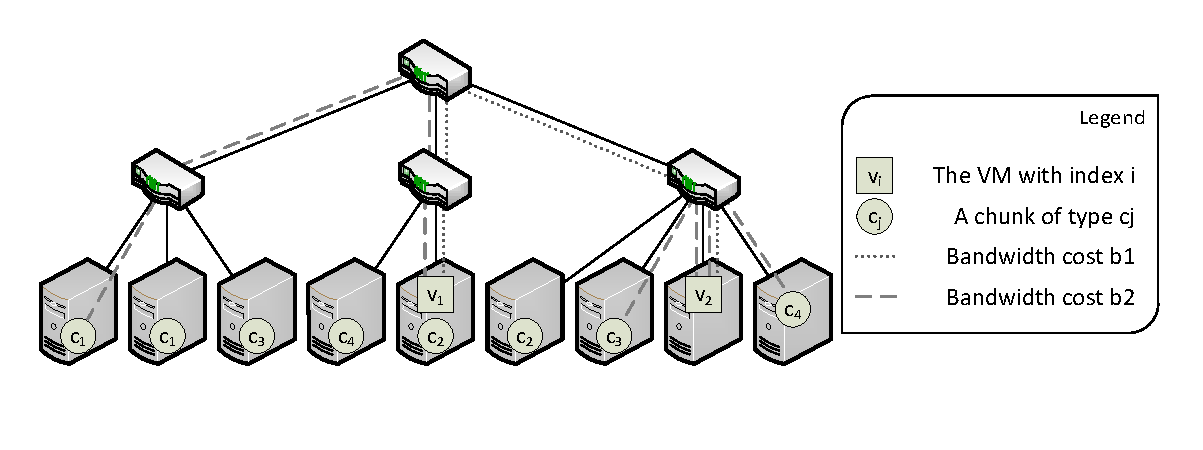
\includegraphics[width=0.99\columnwidth]{figs/overview-fig.pdf}
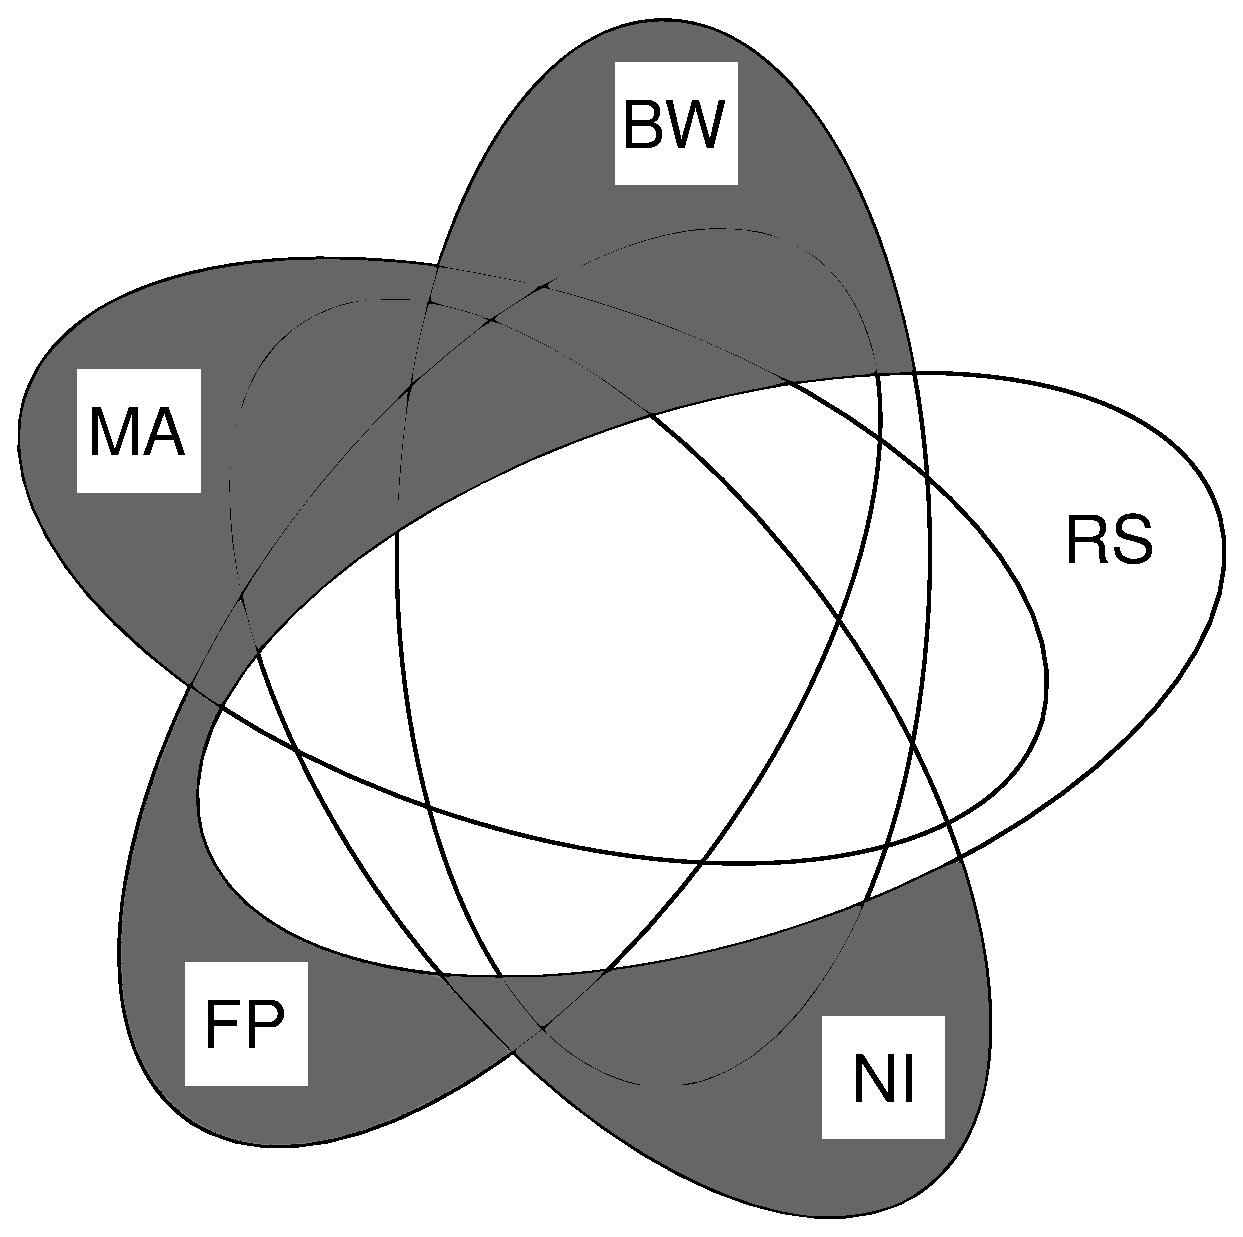
\includegraphics[width=0.49\columnwidth]{figs/venn_dp.pdf}
\caption{Variants solved by dynamic programming approach.}
\vspace{-1em}
\label{fig:venn_flow}
\end{figure}

Figure~\ref{fig:dynamic_motivation} \emph{(right)} shows a different node
mapping~$\NodeMapping_2$, which seeks to minimize the communication costs
between the nodes, and places all nodes in one subtree. The distance between all
nodes is two, which results in a total bandwidth allocation of~$12\cdot\CostCom$
for the interconnect. However, this reduced price comes at additional costs in
the access network:~$c_3$ and~$c_4$ have to be communicated to~$v_3$ and~$v_4$,
which requires a total bandwidth allocation of~$8 \cdot \CostTrans$.


\begin{figure}
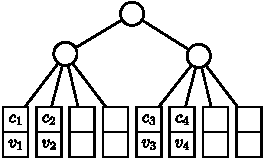
\includegraphics[width = 0.49\columnwidth]{figs/dynamic_bad}
\hfill
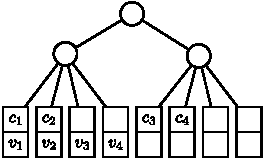
\includegraphics[width = 0.49\columnwidth]{figs/dynamic_good}
\caption{Two different node placements for the same substrate graph and chunk
locations. For~$\CostTrans = \CostCom$, both solutions have an identical
footprint. In other cases, one solution outperforms the other.}
\label{fig:dynamic_motivation}
\vspace{-1em}
\end{figure}



\textbf{Basic ideas.} Our proposed approach is based on dynamic programming, and
leverages the \emph{optimal substructure property} of~$\MA+\FP+\CC+\BW$:
as we will see, optimal solutions for subproblems (namely subtrees)
can efficiently be combined into optimal solutions for larger problems.
Indeed, the~$\MA+\FP+\CC+\BW$ problem
exhibits such a structure, and we show how to exploit it to
compute efficient embeddings, even in scenarios where multiple chunks
need to be assigned to flexibly placeable nodes.

For ease of presentation we will transform the
substrate network~$\Tree$
into a binary tree, using binarization:
we clone every higher-degree node,
iteratively attaching additional clones as right children
and original children as left descendants.
%Last child is placed as
%right son of last clone.

As usual in dynamic programs, we define, over the structure of the tree, a
recursive formula~$f$ for
the minimal cost solution \emph{given} any possible number of nodes
embedded in a given subtree. The actual set does not matter,
due to symmetry arguments.
Our approach is to evaluate this function in a bottom-up
manner.
To finally compute the actual optimal embedding,
we traverse the computed minimal-cost path backwards
(according to
the optimal values found for~$f$ during the bottom-up computation).

Concretely, the first argument to function~$f$
is a subtree~$\Tree'$, containing a given number of
chunks~$\ChunkCount(\Tree')$,
and the
second argument is the number of nodes to be embedded in the subtree.
Function~$f$ is evaluated in a bottom up manner. We initialize the
function at each leaf~$\ell$, by~$f(T_{\ell},x) =
\infty$ for all numbers of nodes~$x$ which are larger than
the server capacity~$\capacity(\ell)$;
to calculate~$f(T_{\ell}, x)$, for~$x \leq \capacity(\ell)$, we compute the
bandwidth allocation on the uplink of~$T_{\ell}$, referred to by the function
$bw(T_{\ell},x)$:
$bw(T_l,x)=  \CostTrans \cdot~$~$|x - \ChunkCount(T_{\ell})| +$~$ \CostCom \cdot
(\Vms - x) \cdot x$,
which accounts for the bandwidth allocation on the uplink of~$T_{\ell}$. The
first
term represents the required bandwidth for the communication between the~$x$
nodes on~$\ell$, and the~$\Vms - x$ nodes in the remaining parts of the substrate
network.
%Obviously the communication~$x$ among the~$x$ nodes within~$T_l$
%does not require bandwidth on the uplink of~$T_l$.
The second term represents
the bandwidth, which is necessary to transport the chunks from their location to
the node which should process the data (see Lemma~\ref{lemma:uplink} for more
details).
%Since placing nodes on servers will not require additional bandwidth
%allocations,~$bw$ is equal to~$f$ on all subtrees~$T_l$, which consist only of
%a single leaf. If the required bandwidth~$bw$ exceeds the avialble bandwidth
%$\capacity$ on the uplink,~$f(T_l,x)$ is set to~$\infty$, to mark the
%corresponding number of nodes in the subtree as infeasible.}

After initialization, we proceed to compute~$f$ for non-leaf
nodes in a bottom-up manner: We split the~$x$ nodes
into two positive integer
values, and we put~$r$ on the right and~$x - r$ on the left subtree.
That is, we take the optimal cost
(given recursively) of placing~$r$ nodes in
the right subtree~$\textsc{Ri}(T')$ of~$T'$ and~$x-r$ nodes in left subtree~$\textsc{Le}(T')$ of
$T'$. Given the cheapest combination, we add the bandwidth requirements
on the uplink of~$T'$ to generate the overall costs for placing~$x$ nodes in~$T'$.
Therefore,~$f(T',x) =   \min_{0\leq r \leq x}$~$ \{  f\left(\textsc{Le}(T'),
x-r\right) +$~$
f\left(\textsc{Ri}(T'), r\right) \} + bw(T',x)$.
Again, we set~$f(T',x)$ to infinity if the required bandwidth
$bw$ exceeds the capacity~$\capacity$ of the uplink of~$T'$.

%This allocation consists of two parts: (1) The node inter-connect
%communication is easy to compute, as we know how many
%nodes are in the left and right subtree, and how many are
%outside.
%Concretely, for each node pair communicating across subtrees we
%charge~$b_2 \cdot (w(e_1) +
%w(e_2))$, for each pair where one is in the subtree and the other outside,
%we charge~$b_2 \cdot
%w(e_1)$. Right subtree case is symmetrical.
%(2) The chunk access cost
%can be computed by greedily matching nodes to chunks locally (first
%inside the subtree, then across subtrees, then outside~$T'$).
%In particular, we can
%just consider the absolute value of the difference between the number of chunks and
%the number of nodes in a given subtree, without knowing which
%is bigger, because in our model if there are some nodes
%left, we know that some chunks from outside will use the same transfer
%as if we have excessive chunks in the subtree.

%Assume there are~$c_{\ell}$ chunks in the left and~$c_r$
%chunks in the right subtree. To incline minimal cost we connect chunks in
%given subtree to nodes in the same subtree. If we can no
%longer do that, because~$v_i < c_i (i \in \{l,r\})$, then we connect
%leftover chunks to nodes in second subtree of~$T$. If we
%can no longer do that, we connect leftover chunks outside of~$T$. This
%strategy is optimal, because connecting any other way can be amended
%(TODO: need better argument here), inclining lower cost. Connections
%inside either left or right subtrees inclines cost~$0$ to edges~$e_1$
%and~$e_2$. Connections between left and right subtree incline cost
%$b_1
%\cdot (w(e_1) + w(e_2))$. Connections from either subtree to outside
%of~$T$ inclines either~$b_1 \cdot w(e_1)$ or~$b_2 \cdot
%w(e_2)$. Finally, we can write down our formula for~$f$:


%

%Therefore, we have:
%\begin{eqnarray*}
%f(T', x) &=& \min_{\ell \in \{0, \ldots, x\}}  f(\textsc{Le}(T'), {\ell}) + f(\textsc{Ri}(T'), x - {\ell}) \\
%&&+ \CostTrans(\textsc{Le}(T'),{\ell},\textsc{Ri}(T'),x-l)\\ &&+ \CostCom({\ell},x-{\ell})\\
%\end{eqnarray*}
%




\textbf{Analysis.}
The correctness and optimality of our dynamic program
is due to the decoupling of the costs induced by the tree
structure of~$\Tree$ and the  substructure
optimality property.
The substructure optimality follows from the observation that
costs can be accounted on the uplink, and the fact
 that we check each possible node distribution.
For each substrate vertex ($n_S$ many) we have
to check the cost of all possible splits,
resulting in an overall complexity of~$\mathcal{O}(n_S \cdot n_V^2)$.
The runtime to binarize~$\Tree$ is asymptotically negligible.

%\textbf{Summary.}
%Figure~\ref{fig:venn_dp} summarizes all problem
%variants which can be solved with our dynamic programming approach.
%\begin{wrapfigure}{r}{0.5\columnwidth}
%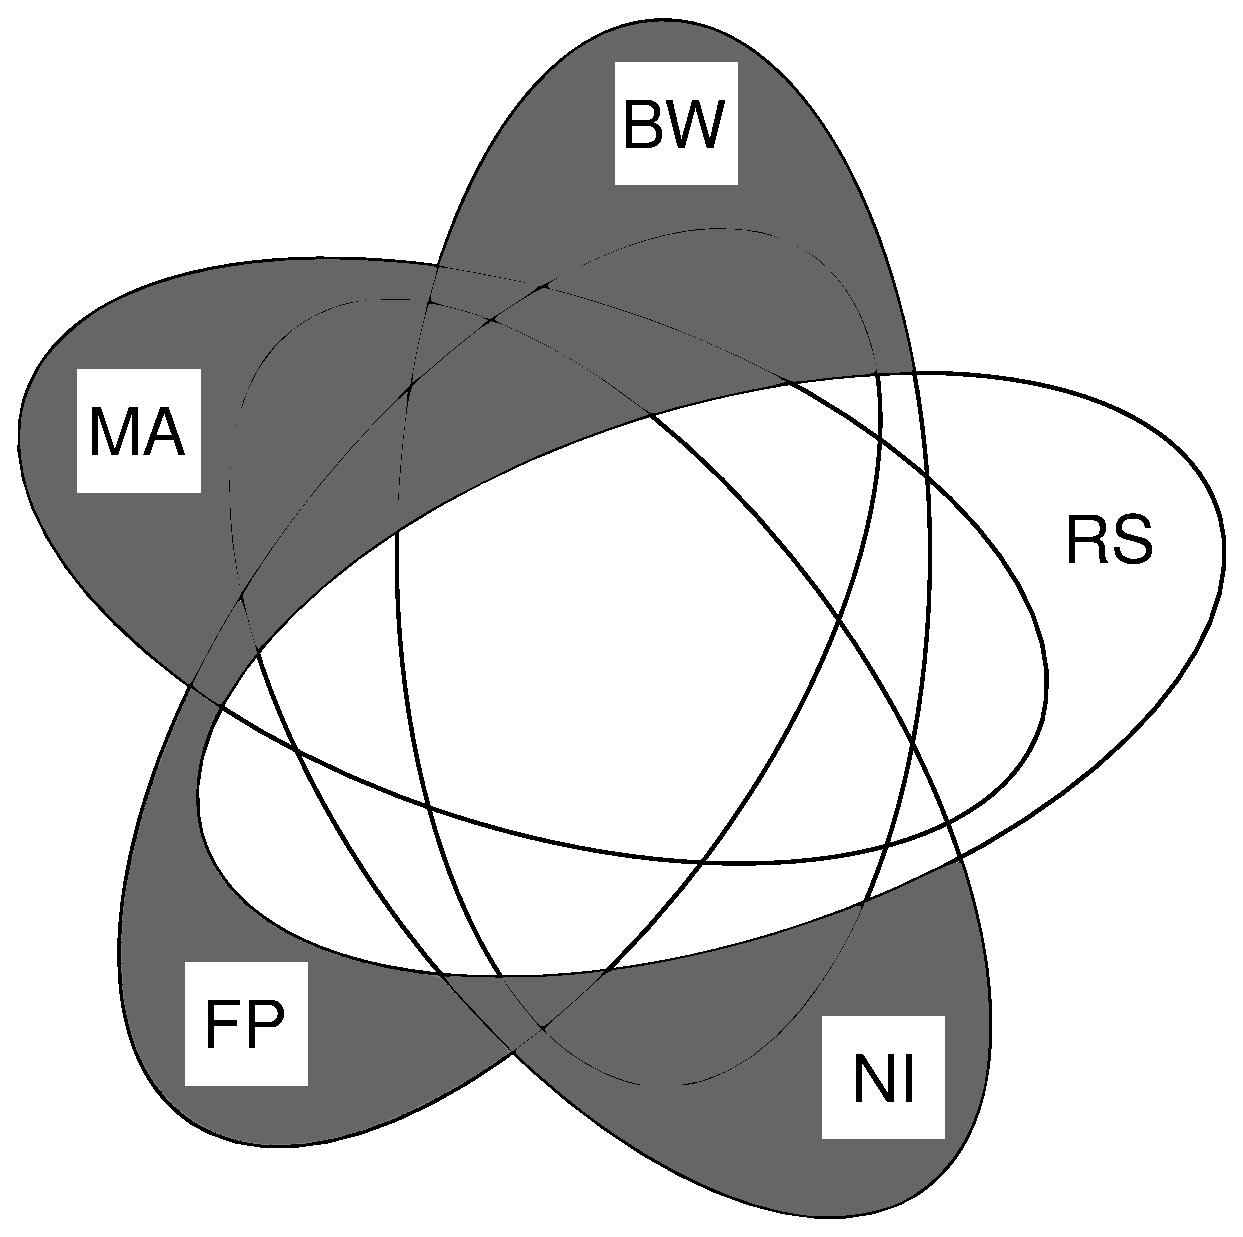
\includegraphics[width=0.48\columnwidth]{figs/venn_dp.pdf}
%\caption{Variants solved by programming approach.}
%\label{fig:venn_dp}
%\end{wrapfigure}



\subsection{Simple Problems}

\begin{figure}
\centering
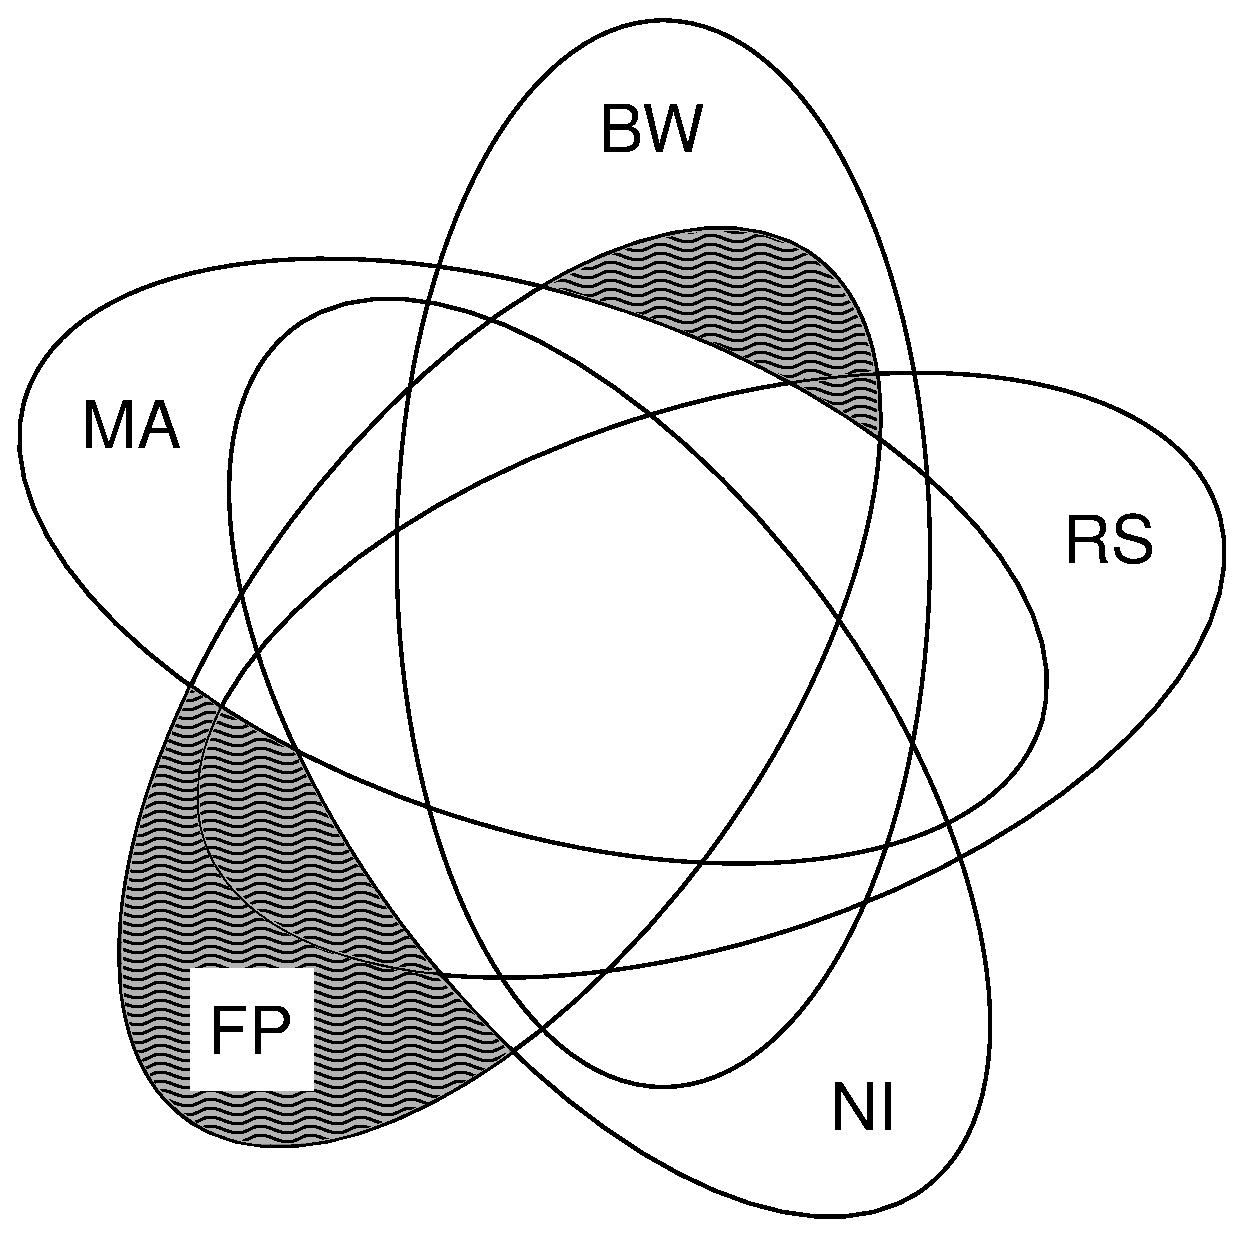
\includegraphics[width=0.49\textwidth]{figs/venn_trivial.pdf}
\caption{Trivially solvable problem variants.}
\label{fig:venn_trivial}
\end{figure}


For the sake of completeness, we also observe that there are
several problems which
allow for a trivial solution. Concretely, problems with~$\FP$
plus any combination of
$\RS$ and~$\BW$ (but without~$\MA$ and~$\CC$) can easily be solved by
mapping
nodes to chunk locations.
Figure~\ref{fig:venn_trivial}
shows a Venn diagram of the trivial property combinations.

%%%%%%%%%%%%%%%%%%%%%%%%%%%%%%%%%%%%%
\section{NP-Hardness Results}\label{sec:np}

We have seen that even problems with multiple dimensions of
flexibility can be solved optimally in polynomial time.
This section now points out fundamental
limitations in terms of computational tractability.
% In particular, we
%will show that problems become NP-hard if multiple chunks have to be
%assigned to a flexibly placeable node ($\FP+\RS+\MA$ is proved NP-hard in
%Section~\ref{ssec:fprsma}), and if inter-connects have to be established
%between flexible nodes ($\FP+\RS+\CC$ is proved NP-hard in Section~\ref{ssec:fprscc});
In particular, we
will show that problems become NP-hard if flexibly placeable nodes ($\FP$) have to be assigned to one of multiple replicas ($RS$), either with multiple chunks per node ($\MA$ in Section~\ref{ssec:fprsma}) or with communication among nodes ($\CC$ in Section~\ref{ssec:fprscc}).
Both results hold even in uncapacitated networks, and even in small-diameter
substrate networks (namely two- or three-level trees~\cite{fattree}).
The hardness of~$\FP+\RS+\MA$ and~$\FP+\RS+\CC$ imply
the hardness of four additional, more general models, as
summarized in Figure~\ref{fig:np_implications}:\\
\begin{figure}[htbp]
\centering
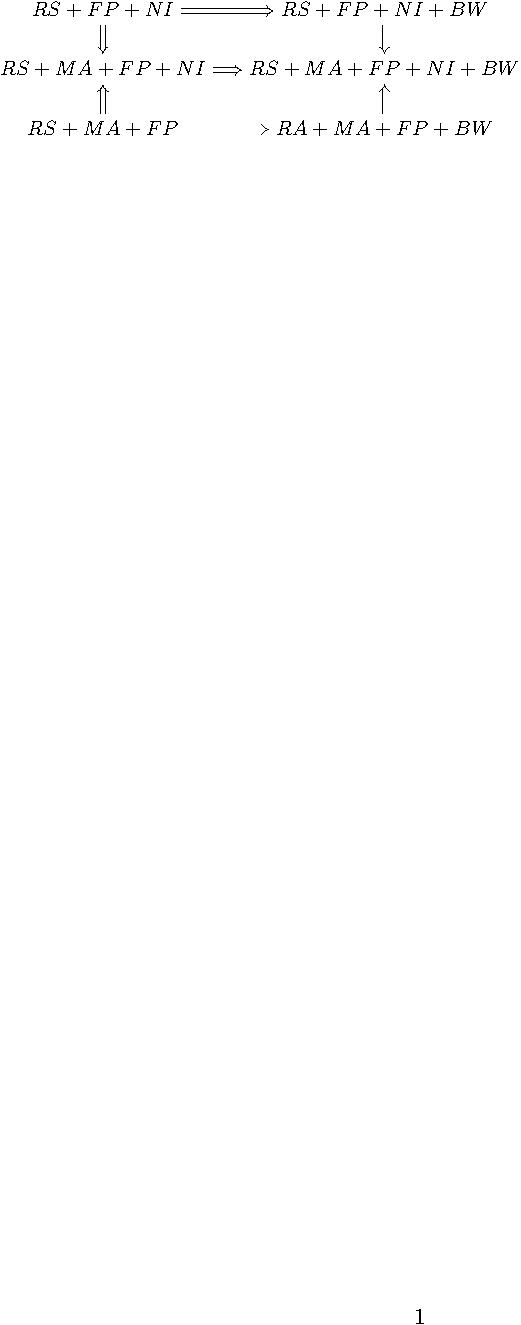
\includegraphics[width = .6\columnwidth]{figs/np_implications}
\caption{The NP-hardness of~$2$ variants implies the hardness of 
$4$ other variants.}
\label{fig:np_implications}
\end{figure}
%Additional NP-hardness results appear in the Appendix.

% Stefan: I agree, but let's do that later, little time right now :-)
%\maciek{I don't like naming the instances I and I'. We want a name that has 3 in it for an instance of perfect matching; we can choose and consistantly use some name for %instance of any VCEMB. This is general comment that applies for both proofs in this section as well as an appendix}.

\subsection{Introduction to 3D Perfect Matching}
\label{sec:3dm_intro}

Both the hardness of~$\FP+\RS+\MA$ and~$\FP+\RS+\CC$ are shown by a reduction
from the NP-complete problem of \emph{3D Perfect Matching}~\cite{3dmatch},
which we can see as a generalization of bipartite matchings to 3-uniform
hypergraphs. We will refer to this problem by~$\TDM$, and for completeness,
review it quickly:
$\TDM$ is defined as follows. We are given three finite and disjoint
sets~$X$,~$Y$, and~$Z$ of cardinality~$k$, as well as a subset of triples~$T\subset
X \times Y \times Z$.  Set~$M \subseteq T$ is a 3-dimensional matching
if and only if, for any two distinct triples~$t_1=(x_1, y_1, z_1) \in M$
and~$t_2=(x_2, y_2, z_2) \in M$, it holds that~$x_1\neq x_2$,~$y_1\neq
y_2$, and~$z_1\neq z_2$. Our goal is to decide if we can construct
a~$M \subseteq T$ which is \emph{perfect}, that is, a subset which covers all
elements of~$X \cup Y \cup Z$ exactly once.


\subsection{Multi-Assignments are hard ($\FP+\RS+\MA$)}\label{ssec:fprsma}

Our proof that~$\FP+\RS+\MA$ is NP-hard is based on the following main ideas.
We encode a~$\TDM$ instance as an~$\FP+\RS+\MA$ instance as follows:

 \begin{itemize}
 \item For every element in the universe~$X\cup Y\cup
 Z$, we create a chunk type. Intuitively, in~$\TDM$,
 each element must be covered, which corresponds to the requirement
 of~$\FP+\RS+\MA$
 that each chunk type is processed.

 \item We will encode each triple as gadget with three leaves in
 a substrate tree~$\Tree$. The three leaves are close to each
 other in~$\Tree$, and the placement of chunk replicas in~$\FP+\RS+\MA$
 corresponds to the elements of the
 triples in these leaves.

 \item The node placement will correspond to the choice of triples,
 independently of which
leaf the node is mapped to.
 A node will process its collocated chunk,
 as well as the chunks in other two leaves of the same gadget.

\item In order to turn the optimization problem into a decision problem, we will use
a cost threshold~$\Thr$. The cost threshold will be met by all
assignments which assign all three chunks of each triple to a
node which is collocated with one of the chunks. Assignments which connect a
chunk to a node in a different triple, will have a larger footprint, and are
considered to be infeasible.

\end{itemize}


\textbf{Construction.}
Given an instance~$I$ of~$\TDM$ in which~$k$ triples have to be
choosen, we construct an instance~$I'$ of
$\FP+\RS+\MA$ as follows:
\begin{itemize}
\item \emph{Tree Construction:} We create a tree consisting of a root,
and for each triple, we create a gadget which we directly attach as
child of the root. The gadget is of height 2,
and has the following form:
The gadget of each triple consists of an inner node (a router) and three leaves.
\item \emph{Chunks and chunk replicas:} For each element in~$X$,~$Y$ and~$Z$,
 we create a chunk type
($3 \cdot k$ in total). Every gadget contains three chunk replicas,
corresponding to the elements of the triple. Each leave in a gadget, contains
exactly one replica.
\item \emph{Other properties:} We set the number of to-be-embedded nodes to~$k$,
$\CostTrans$ to~$1$, and the number of chunk slots in each node to the multi-assignment factor
$\MaFactor=3$.
%\stefan{what
%is the number of slots here?}\maciek{it is number of replicas that
%each VM can process (the MA property)}.
We use a threshold~$\Thr= 4
\cdot k$.
% \maciek{If we update the model to take care of hosting
%  multiple VMs in one leaf, we should set this instance to allow only
%  one VM per leaf. However, any number of VMs per leaf will be OK for
%  this proof.}
\end{itemize}

\textbf{Example.} Figure~\ref{fig:fprsma} shows an example of our construction: An
instance~$I$ of 3-DM is given: The disjoint sets~$X$,~$Y$ and~$Z$ have a
cardinality~$k=2$. We will refer to the two elements in~$X$ as~$x_1$ and~$x_2$,
and use the same notation for the other two sets.~$T$ contains the three triples
$(x_1, y_1,
z_1)$,~$(x_2, y_1, z_2)$, and~$(x_2, y_2, z_2)$. The goal of 3-DM is to find a
subset~$M \subseteq T$, which contains each element in each of the three sets
exactly once. This instance only has one solution:~$M =
\{(x_1,y_1,z_1),(x_2,y_2,z_2))\}$.

To construct the corresponding instance~$I'$ of~$\FP+\RS+\MA$, we
create a gadget for each triple in~$T$. For each variable which occurs in a
triple, the corresponding gadget contains a chunk of the
type of the variable. The triple
$(x_2, y_1, z_2)$ of the instance is represented by the middle gadget in
Figure~\ref{fig:fprsma}. The objective of~$I'$ is to spawn~$k=2$ nodes,
with the smallest possible footprint. If the total footprint is~$\leq
2\cdot2\cdot k$, we can construct a solution to~$I$ from the solution to~$I'$.
The footprint consists of the costs which occur when a node is embedded in a
gadget, and the three chunks of that gadget which are assigned to that node: one of
the chunks is collocated with the node, the other two have to be transferred
via two hops, inflicting unitary costs on each hop.
%\begin{figure}[htbp]
%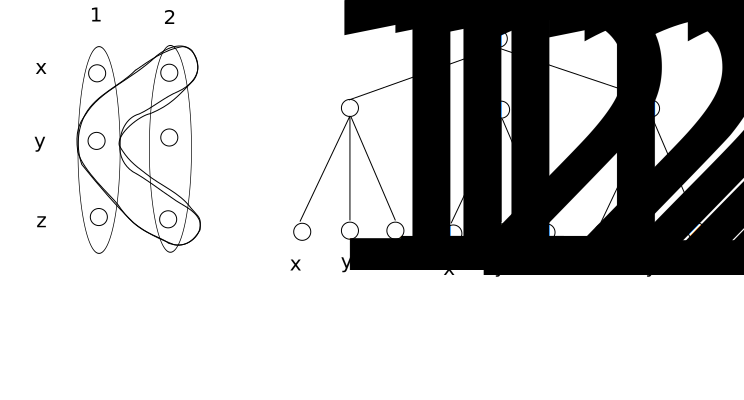
\includegraphics[width = \columnwidth]{figs/example-matching}
%\end{figure}
\begin{figure}[t]
\includegraphics[width = 0.3\columnwidth]{figs/np_3dm_formular}
\hfill
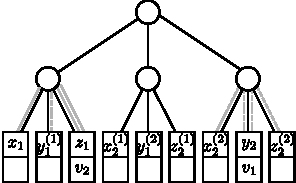
\includegraphics[width = 0.6\columnwidth]{figs/np_3dm_construction}
\caption{\textit{Left:} A~$\TDM$ instance with three triples:
$(x_1, y_1, z_1)$,~$(x_2, y_1, z_2)$, and~$(x_2, y_2, z_2)$. The solution is
indicated by the grey triples; the dashed triple is not used for the
solution. \textit{Right:} The corresponding problem and solution of~$\FP + \MA
+ \RS$.}
\label{fig:fprsma}
\end{figure}


\textbf{Correctness.}
Given these concepts, we can now show the computational hardness.
\begin{theorem}
$\FP+\RS+\MA$ is NP-hard.
\end{theorem}
\begin{proof}
Let~$I$ be an instance of~$\TDM$ and let~$I'$ be an instance of
$\FP+\RS+\MA$ constructed as described above. We prove that~$I'$ has a solution of cost~$\leq \Thr$ if ($\Rightarrow$) and only if
($\Leftarrow$)
$I$ has a matching of size~$k$.

($\Rightarrow$) Let us take a solution to~$\TDM$. We place a node in every
gadget that corresponds to the chosen triples. In each of the corresponding
gadgets, we match every chunk to the node in this gadget. This
solution has
cost exactly~$\Thr$. As every element of the universe is covered, every
chunk type is processed.

($\Leftarrow$) Let us take a solution to~$\FP+\RS+\MA$ of cost~$\leq \Thr$. We
choose triples that correspond to gadgets where there are nodes. Since
all chunks are processed, every element of~$X$,~$Y$ and~$Z$ is matched. Each
node must process chunks that
correspond to the triple, otherwise the
cost must be larger than~$\Thr$ (high costs for chunk
transportation).
\end{proof}


\subsection{Inter-connects are hard ($\FP+\RS+\CC$)}\label{ssec:fprscc}


Next, we prove that the joint optimization of node placement and replica selection
is NP-hard if an inter-connect has to be established between nodes.
In our terminology, this is the~$\FP+\RS+\CC$ problem.

The proof is similar in spirit to the proof of~$\FP+\RS+\MA$, however,
we modify the construction to account for the absence of~$\MA$:
we choose
a high value for~$\CostTrans$, such that nodes will be directly collocated with
their assigned chunks. We leverage the fact that any solution which does not
assign 0 or 3 chunks to each gadget, will have higher communication costs.

\textbf{Construction.}
Let~$I$ be an instance of~$\TDM$. We will create an instance~$I'$
for~$\FP+\RS+\CC$ as follows:
\begin{itemize}
\item We will construct the same tree as in previous reduction with
chunk replicas placed in the same way.
\item The communication cost in the inter-connect is set to~$\CostCom = 1$.
\item The number of nodes (virtual machines) is~$\Vms = 3 \cdot k$, where~$k$ is the set cardinality.
\item Only solutions which place a node in each leaf of~$k$ gadgets, can
be converted into solutions for the 3-DM problem. We use the cost threshold
$\Thr =  6 \cdot k + 18 \cdot
(k - 1) \cdot k$, to verify whether a solution achieves this, transforming
$\FP+\RS+\CC$ into a decision problem. A detailed explanation of this value can
be found in the proof of Theorem~\ref{theorem:fp_rs_cc}.
%\maciek{If we update the model to take care of hosting
%  multiple VMs in one leaf, we should set this instance to allow only
%  one VM per leaf. In this proof it also does not matter, as it is
%  already forced by infinite transportation cost, however we need to
%  define it anyway.
%  }
\item We set the access cost~$\CostTrans$ to a chunk replica to a high value~$W$. This will force
nodes to be collocated with the replica. One example of sufficient
(and polynomial but not necessarily minimal)~$W$
is the value of the threshold~$\Thr+1$. Any solution not
assigning chunks to collocated nodes, have cost~$> \Thr$:
communicating a chunk inflicts costs~$W=\Thr+1$ over every link.
\end{itemize}

We focus on instances with unit server capacities.

\textbf{Proof of correctness of the reduction.}
Intuitively, in order to minimize embedding costs,
nodes should be placed on near-by replicas. We use the following
helper lemma.
\begin{lemma}\label{lemma:helper}
In every valid solution of~$I'$ of cost~$\leq \Thr$, each gadget
falls in one of two categories:
$k$ gadgets have exactly
$3$ nodes, and~$n-k$ gadgets remain empty.
\end{lemma}
\begin{proof}
Since~$W$ is large enough, the~$3\cdot k$ nodes have to be placed
directly on different chunks, resulting in 0 costs for the access network.
Consider any pair of nodes
communicating over the
inter-connect; due to our construction, the communication cost
for each such pair is either
2 hops (if they belong to the same gadget) or 4 hops (if they belong
to different gadgets).
The lemma then follows from the observation that~$\Thr$
is chosen such that it is never possible to distribute nodes
among more than~$k$ gadgets.
\end{proof}

\begin{theorem}
\label{theorem:fp_rs_cc}
$\FP+\RS+\CC$ is NP-hard.
\end{theorem}
\begin{proof}
Let~$I$ be an instance of~$\TDM$ and let~$I'$ be an instance of
$\FP+\RS+\CC$ constructed as described above.
We prove that~$I'$ has solution of cost~$\leq \Thr$ if ($\Rightarrow$) and only if
($\Leftarrow$)
$I$ has a solution.

($\Rightarrow$) In order to compute a solution
for~$I'$ given a solution for~$I$, we proceed as follows.
Given an exact covering set of triples~$S = \{t_1, t_2,
\ldots, t_k\}$, we place three nodes in each gadget that
corresponds to every triple of~$S$. Chunks are matched to the nodes which are located
on the same server.

The solution has the following cost:
(1) the communication cost inside a gadget is~$2 \cdot {3 \choose 2}$,
  as every pair contributes two hops;
  (2) the communication cost from each gadget to all other gadgets is~$4
  \cdot 3 \cdot 3 \cdot (k - 1) / 2$, where the factor~$4$ is
  for the
  communication over~$4$ hops, the factor~$3$
  corresponds to the number of nodes per gadget, and
 ~$3 \cdot (k-1)$ is the number of nodes in remote gadgets;
  as we count each pair twice, we need to divide by two in the end.
Summing up over all~$k$ gadgets, we get exactly~$\Thr$.

($\Leftarrow$) Given a solution for~$I'$,
we can exploit Lemma~\ref{lemma:helper} to construct a solution for~$I$.
We know that in any solution of cost at most~$\Thr$,
$k$ gadgets contain exactly 3 nodes. These gadgets correspond to a valid
3D Perfect Matching: exactly one replica of every chunk type is processed and
hence every element is covered exactly once.
\end{proof}

%Finally, let us conclude by remarking that all NP-hard problems discussed in this paper
%are obviously also in NP (and hence NP-complete): solutions can be verified efficiently.


\section{A Detailed Study of Replica Selection Hardness}\label{ap:tworep}

We have seen that replica selection flexibilities can render embeddings computationally hard.
We will now provide a more detailed look at this hardness result
and explore the minimal requirements for rendering replica selection hard.
In particular, we will show that already two replicas for each chunk type are sufficient to
introduce intractability.

Across the next sections, we use the following notation:

\begin{enumerate}
  \item $n := |X|$ (remember that $|X| = |Y| = |Z|$)
  \item $e$ -- an element of the universe ($e \in X \cup Y \cup Z$)
  \item $T$ -- set of triples
  \item $t = |T|$
  \item $T_e$ -- set of triples that contain element $e$
  \item $\deg(e) := |T_e|$
  \item $\lbrace e_X(\tau), e_Y(\tau), e_Z(\tau) \rbrace$ -- elements of triple $t$
  \item $V$ -- set of nodes to be spawned in embedding instance
\end{enumerate}

\subsection{Two Replicas without Bandwidth Constraints}

We now show that the 2-replica selection problem is even NP-hard
without capacity constraints.  In particular, we consider the problem
variant~$\RS(2)+\MA(4)+\FP$ with at most two replicas of each chunk type and assignment factor
four. There are no capacity constraints on links.

\textbf{Construction.}

Let's take any instance~$I_{\TDPM}$ of~$\TDM$ and create a~$\RS(2)+\MA(4)+\FP$
instance~$I_{\VCEMB}$ as follows.

\paragraph{Chunks}

We construct three types of chunks. The first type corresponds to covers of elements by triples, with two replicas each. The other two types are chunk types with one replica only, therefore called \emph{unique}. We construct two types of unique chunks, distinguished by a different role in the construction. For unique chunks we simply annotate the chunk type with chunk replica.
Thus, the constructed instance uses at most two replicas of each chunk type.

\begin{enumerate}
  \item For each triple $\tau \in T$, we construct $3$ chunk types, with two replicas each. We construct different chunk types for each triple $\tau$, which 
  contain element $e$. We refer to those replicas by $ch_1(e, \tau)$ and $ch_2(e, \tau)$.
  \item We construct~$n$ additional chunk types named
  ~$u_1, \ldots, u_n$, with one replica each.
  \item For each element~$e\in X\cup Y\cup Z$,
  we construct additional~$3\cdot(\deg(e) - 1)$ chunks, with one replica each.
  We call this set~$\UniqueE$.
\end{enumerate}

\paragraph{Tree}

We construct the following tree.

\begin{figure}[t]
  \centering
  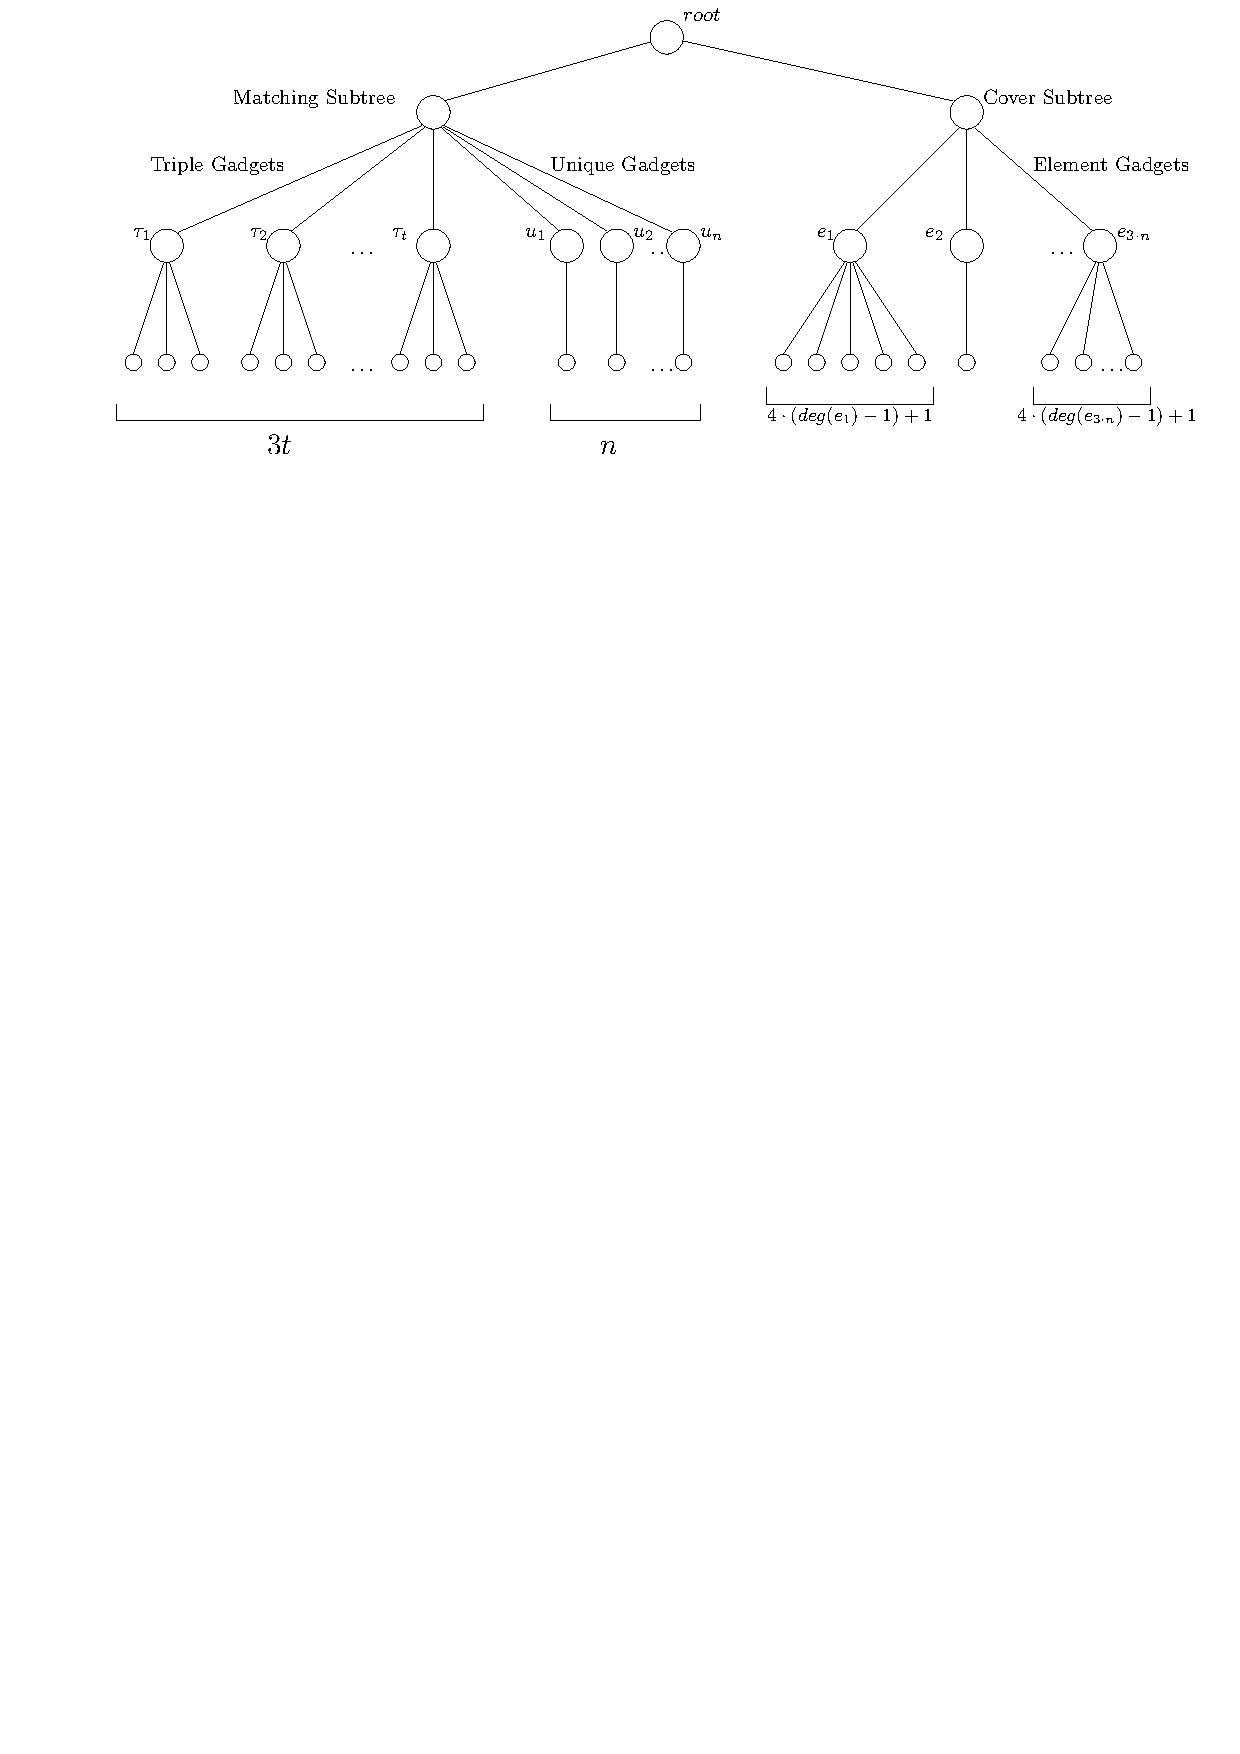
\includegraphics[width=0.99\columnwidth]{reduction/overview.pdf}
  \vspace{-1em}
  \caption{Overview of the substrate network}
  \vspace{-1em}
\end{figure}


\begin{enumerate}
  \item The physical network consists of two subtrees connected to the
  root: A {\MatchSubtree} and a {\CoverSubtree}. The
  {\MatchSubtree} consists of $|T|$ {\TripleGadgets}, one per each triple $t\in T$ and $n$
  {\UnqGadgets}. The {\CoverSubtree} consist of~$n$ {\ElGadgets}, one for each element $e\in X\cup Y\cup Z$.
  \item {\TripleGadget} consists of four vertices: three leaves and the root of the gadget.
  \item {\UnqGadget} consists of two vertices: the leaf and the root of the gadget. Note that we construct
  nodes not only to keep the tree balanced, but also to keep leaves of
  {\UnqGadgets} far from leaves of other \UnqGadgets.
  \item {\ElGadget} of element $e$ has a structure that depends on the number of triples that cover $e$. The {\ElGadget} consists of the
  root, and~$4\cdot(\deg(e)-1)+1$ leaves.
\end{enumerate}

\paragraph{Chunk Placement}
The chunks are placed as follows:
\begin{enumerate}
  \item \emph{Chunks in matching subtree:} In {\TripleGadget} of triple $\tau$ we put
  three replicas:
 ~$ch_1(e_X(\tau), \tau), ch_1(e_Y(\tau), \tau), ch_1(e_Z(\tau), \tau)$, one per each leaf.
  \item \emph{Chunks in unique subtree:} We place replicas
 ~$u_1,\ldots, u_n$ at the leaves of \UnqGadgets.
 \item \emph{Chunks in element gadget:} In leaves {\ElGadget} of element $e$ we put replicas $ch_2(\tau, e)$ for each $\tau \in T_e$. Additionally, we put replicas $\UniqueE$.
\end{enumerate}

\paragraph{Other properties of the instance}
\begin{enumerate}
  \item \emph{Multiple assignment:} We set the assignment factor (number of processed
  chunks by each node) to four.
  \item \emph{Number of nodes:} We allow to spawn
 ~$\numNodes := n + \sum_{e}(\deg(e)-1)$ nodes.
  \item \emph{Threshold:} We set the following threshold for cost of a solution to be feasible.
 ~$\Thr := 8\cdot n + 6\cdot\sum_{e}(\deg(e)-1)$
\end{enumerate}


\textbf{Reduction.}  We can make the following observations.

\begin{obs}
  The construction fulfills the following properties:
  \begin{enumerate}
    \item There is exactly one replica of each chunk type (except\hspace{1mm} $\UniqueE$ for each edge $e$) in the
    \MatchSubtree.

    \item There is exactly one replica of each chunk type in the
    \CoverSubtree.

    \item There are at most two replicas of each chunk type in the
    substrate network.
  \end{enumerate}
\end{obs}

For the reduction we proceed as follows:
\begin{enumerate}
  \item Let's take any instance $I_{\TDM}$ of $\TDM$ and produce an instance $I$ as described in the construction section.
  \item Let's take any feasible solution $S_{\TDM}$ to $I_{\TDM}$ and place $n$ (remember that~$n=|X|=|Y|=|Z|$) nodes in the following way: for each triple $r$ chosen in $S_{\TDM}$ solution, we select an arbitrary leaf of the Triple Gadget corresponding to $r$ and place a node there.
  We
  match each such node to three chunks that are put in its
  {\TripleGadget} (it is co-located with one of the chunks), and we match it to an
  arbitrary unmatched chunk in any \UnqGadget.
  \item We put~$\deg(e)-1$ nodes in each \emph{Element Gadget}. We match all
  remaining chunks from this \emph{Element Gadget} to those nodes in an
  arbitrary way.
  \item This solution has cost~$\leq \Thr$ (easy to see by summing up the
  costs of transporting chunks to each node).
  \item The feasibility of the constructed solution follows from the
  fact that each chunk type was processed; each node processes four
  chunks.
\end{enumerate}

\textbf{Proof of correctness of the reduction.}

Before we start the reduction, let us introduce two functions that will help us show that certain node placements are infeasible, as their cost exceeds the threshold.
  For each $u \in \{ 1, \ldots, t-1 \}$ let us define
 ~$\CostEstimOne(u) = u \cdot 12 + (\tau-u)\cdot 4 + (4\cdot n -
  n - 4\cdot u - (\tau-u))\cdot 2$, and 
$\CostEstimTwo(u) = 4\cdot \tau + (4\cdot
n - n - \tau)\cdot 2$, where $\tau$ is the number of triples and $n = |X| = |Y| = |Z|$ in a given instance of $\TDM$.
We use the function $\CostEstimOne(u)$ in Lemma~\ref{th:no-unique} to show that no node spawned in the Unique Subtree: the $\CostEstimOne(u)$ is the lower-bound on the total cost of the solution, assumming that $u$ nodes spawned in the Unique Subtree.
By Lemma~\ref{lem:cost-estims}, for non-zero $u$ the cost lower-bound already exceeds the threshold.
and we use the function $\CostEstimTwo$ in Lemma~\ref{th:np-balance} to show that exactly $n$ nodes spawned in the Matching Subtree. \maciek{After fixing the proof np-balance, write what $u$ corresponds to}

\begin{lemma}
  For each $u \in \{ 1, \ldots, t-1 \}$ we have that $\CostEstimOne(u) > \Thr$ and
  $\CostEstimTwo(u) > \Thr$.
  \label{lem:cost-estims}
\end{lemma}

\begin{proof}
  We have that $\CostEstimOne(u+1) \geq \CostEstimOne(u)$ and $\CostEstimTwo(u+1) \geq \CostEstimTwo(u)$ , for
 ~$1\leq u \leq t-1$. It is easy to verify that $\CostEstimOne(1) > \Thr$ and $\CostEstimTwo(1) > \Thr$.
\end{proof}

\begin{lemma}
  Take any feasible solution~$\Solution$ to the instance~$I$ of
 ~$\RS(2)+\MA(4)+\FP$ (as constructed above). If the cost of
 ~$\Solution$ is at most~$\Thr$, then no node is spawned in the Unique
  Subtree.
  \label{th:no-unique}
\end{lemma}

\begin{proof}
  For the sake of contradiction, let us assume a feasible solution
 ~$\Solution$ with at least one node spawned in {\UnqSubtree}. We show
  that in this case, the cost of solution~$\Solution$ is greater than
 ~$\Thr$. Let $\ell$ be the number of nodes spawned in the {\UnqSubtree}. We know
  that~$1 \leq \ell \leq |T|$.  In~$\Solution$ we have exactly
 ~$4 \cdot \numNodes$ chunk transportations, incurring cost
 ~$0, 2, 4$ or~$6$ (the tree has an edge-height of~$3$). At most
 ~$\numNodes$ transportations are of cost~$0$. Note that the leaves of the
  {\UnqSubtree} are separated from other leaves of the tree by at
  least~$4$ edges.  The cost of chunk transportation to nodes
 ~$v \in \SpawnedUnqSubtree$ is at least~$12$. The chunks in
  {\UnqSubtree} are unique, therefore the solution transports~$|T| - \ell$
  chunks to nodes outside the \UnqSubtree, incurring cost~$4$ for each
  chunk.
  Therefore $\CostSol \geq \CostEstimOne(\ell)$, and by Lemma \ref{lem:cost-estims}
  we conclude that $\CostSol > \Thr$.
\end{proof}



\begin{lemma}
  Given any feasible solution~$\Solution$ to a given instance~$I$ of
 ~$\RS(2)+\MA(4)+\FP$ (as constructed above). If the cost of
 ~$\Solution$ is at most~$\Thr$, then exactly~$n$ nodes are spawned in the
  \MatchSubtree.
  \label{th:np-balance}
\end{lemma}
\begin{proof}
    \maciek{This proof requires revision}
  Let~$\ell$ be the number of nodes spawned in
  {\MatchSubtree}.  Let us assume the contrary, namely that
 ~$\ell \neq n$.  First, we use
  Theorem~\ref{th:no-unique} to restrict the placement of nodes in
  \UnqSubtree. Then we consider two cases:
  \begin{enumerate}
    
    \item~\textbf{Case $\ell \leq n$:} There are at least
   ~$u := 4 \cdot (n-\ell)$ chunks in the {\MatchSubtree} that are not
    processed in the {\MatchSubtree}, each incurring transportation
    cost of~$6$.
     From the structure of the substrate network and placement of
    chunks we know that~$\CostSol \geq \CostEstimTwo(\ell)$, and by Lemma \ref{lem:cost-estims}
  we conclude that $\CostSol > \Thr$.
.

    \item \textbf{Case $\ell>n$:} We use the fact that there are not enough nodes in
    {\CoverSubtree}, and we need to transport over~$6$ hops at least 3
    unique chunks for each node missing from {\CoverSubtree}.
  \end{enumerate}
\end{proof}

\begin{theorem}
 ~$\RS(2)+\MA+\FP$ is NP-hard.
\end{theorem}

\begin{proof}
  
  Let's take an instance~$I$ of~$\TDPM$ and construct an instance~$I'$
  of~$\RS(2)+\MA+\FP$ in the way described in the construction section.  We show that~$I'$
  has a solution of cost~$\leq \Thr$ if and only if~$I \in \TDPM$ (there
  exists a perfect 3D matching).

  ($\Leftarrow$) Let's take any feasible solution~$\Sol$ to~$I$. We
  construct a solution~$\Sol'$ to~$I'$ in the following way:
  \begin{enumerate}
    \item We place~$n$ nodes in~$n$ {\TripleGadgets} (one per gadget)
    that correspond to triples in~$\Sol$. We match each such node
    to chunks in the gadget it is placed, as well as one arbitrary
    chunk in {\UnqSubtree}.
    \item In each {\ElGadget} that corresponds to element~$e$, we place
   ~$\deg(e) - 1$ nodes and match them to arbitrary chunks in this
    gadget, which are not yet matched in any {\TripleGadget}.
  \end{enumerate}

  We can observe that every chunk type was processed. By simple
  calculations we see that~$\Sol'$ indeed has cost~$\leq \Thr$.

  ($\Rightarrow$) Let's take any feasible solution~$\Sol'$ to~$I'$.
  We construct the solution~$\Sol$ to~$I$ in the following way:
  We call the {\TripleGadget} \textit{active}, if they contain a node
  at any leaf. We call active node in
  {\TripleGadgets} \ActiveNodes. We construct a~$\TDPM$ solution from
  triples that correspond to active \TripleGadgets.
  We observe the following properties of~$\Solution$:
  \begin{enumerate}
    \item From Lemmas~\ref{th:no-unique} and~\ref{th:np-balance}, we
    know that exactly~$n$ {\TripleGadgets} are \emph{active}.
    \item In~$\Solution$, only one node is spawned in an active
    \TripleGadget.
    \item Each {\ActiveNode}~$v$ processes the 3 chunks that are
    placed in~$v$'s \TripleGadget, as well as one chunk in an \UnqGadget.
    \item Every chunk type is covered.
    \item In each {\ElGadget} for element~$e$, one chunk instance of
    set~$t(e)$ is not processed. Let's call this chunk instance
   ~$\Unmatched(e)$, and let's call
   ~$\Unmatched = \cup_e \Unmatched(e)$. Note that 
   ~$|\Unmatched| = n$.
    The set~$\Unmatched$ is covered by \ActiveNodes
  \end{enumerate}

  From above observations we conclude that~$M_S$ is indeed feasible.
\end{proof}

\subsection{Two replicas without multiple assignment}

We now show that~$\RS(2)+\FP+\CC+\BW$ is even NP-hard without multiple
assignment.

\noindent \textbf{Construction.}

\emph{Chunk Types.}  We construct the following chunk types: For each
element~$e\in X\cup Y\cup Z$, we construct~$\deg(e)$ chunk types with
two replicas. Additionally, we construct
$\max\{3\cdot |T| + 3\cdot n + 1, \sum_e(2\cdot \deg(e)-1)\}$
chunk types called \emph{unique chunks}. We
refer to the set of unique chunks by~$U$.

\emph{The substrate network.}

\begin{enumerate}
  \item The physical network consists of three subtrees connected to
  the root: A {\MatchSubtree}, a {\CoverSubtree}, and a
  {\UnqSubtree}. In the {\MatchSubtree} we put $|T|$
  {\TripleGadgets} (remember that~$|T|$ is the number of triples in
  {\TDPM} instance). {\CoverSubtree} consist of~$n$ element gadgets.
  \item The {\UnqSubtree} consist of~$|U|$ leaves, and two middle nodes:
  a lower and an upper middle node. Note that this is different from $\RS(2)+\FP+\MA(4)$ NP-completeness proof, where {\UnqSubtree} was placed in the {\MatchSubtree}.
  \item \TripleGadget: For each triple, we create a subtree
  consisisting of four vertices: three leaves and one triple root.  We
  attach the root of the triple to the root of the matching subtree.
  \item \ElGadget: For each element~$e \in X\cup Y\cup Z$, we
  construct a subtree consisting of the root of the element (attached
  to the root of the cover subtree), and~$4\cdot(\deg(e)-1)+1$ leaves.
\end{enumerate}

\emph{Chunk placement.}
The chunks are placed as follows:
\begin{enumerate}
  \item \emph{Chunks in matching subtree:} For each triple~$\tau$ we put
  three chunks at the leaves of the corresponding \TripleGadget,
 ~$e_1(\tau), e_2(\tau), e_3(\tau)$.
  \item \emph{Chunks in unique subtree:} We place unique chunks~$U$ at
  the leaves of {\UnqSubtree}.
  \item \emph{Chunks in element gadget:} For each element
 ~$e\in X\cup Y\cup Z$, we place the chunks~$\tau(e)$ at the leaves of
  each Element Gadget.
\end{enumerate}


\emph{Bandwidth constraints.}
We use bandwidth constraints of the form
$\Band(k) := k\cdot(\numNodes - k)$. Namely, we set the bandwidth
constraints of an uplink of an {\ElGadget} for each element~$e$ to 
$\Band(\deg(e)-1)$, the bandwidth of an uplink of a~$\MatchSubtree$ to 
$\Band(n)$, and an uplink of a~$\CoverSubtree$ to 
$\Band(\sum_e (\deg(e)-1)$.

\emph{The threshold value and other properties of the instance.} We set the
cost threshold for any solution to the following value:

\begin{tiny}
\begin{align*}
  \Thr  & = 2\cdot (3\cdot \numNodes + \sum_e (\deg(e) - 1)) & \mbox{(over 2 hops)}\\
        & + 4\cdot (n\cdot (3 \cdot (3\cdot \numNodes - 3)) / 2) & \mbox{(over 4 hops in {\MatchSubtree})}\\
        & + 4\cdot (\sum_e((\deg(e) - 1)\cdot (\sum_{f\neq e} \deg(f) - 1)/2)) & \mbox{(over 4 hops in {\CoverSubtree})}\\
        & + 6\cdot (3\cdot \numNodes \cdot \sum_e(\deg(e) - 1)) & \mbox{(between {\MatchSubtree} and {\CoverSubtree})} \\
        & + |U|\cdot (|U|-1)/2 & \mbox{(inside {\UnqSubtree})} \\
        & + |U| \cdot (3\cdot n + \sum_e (\deg(e)-1) & \mbox{({\UnqSubtree} to other nodes)} \\
\end{align*}
\end{tiny}

  We
set~$\CostTrans$, the cost of chunk transportation to $\Thr+1$ (so that no chunk transportation happens in any feasible solution), 
$\CostCom = 1$, and we host only one node per machine. We set the
number of machines to spawn to:
$\numNodes := 3\cdot n + \sum_e (\deg(e)-1) + |U|$.
\\

\noindent \textbf{Properties of the substrate network.}
\begin{lemma}
  Assume we have a~$\RS(2)+\FP+\CC+\BW$ instance~$I$ with a subtree
 ~$T'$ with~$l$ leaves and the bandwidth capacity on uplink of~$T'$ is
 ~$\Band(k)$. Assume that no chunk transportation is allowed
  ($\CostTrans = \infty$, so every node must be collocated with the
  chunk it processes in every feasible solution), and~$\CostCom = 1$.
  Then in any feasible solution the number of nodes spawned in~$T$ (we
  name it~$s$) satisfies~$s \leq k \vee n-s\leq k$, and~$s \leq l$.
  \label{lem:bandwidth1}
\end{lemma}

\begin{proof}
It holds that ~$s\leq l$ as we cannot spawn more nodes than leaves.
  The bandwidth allocation on the uplink of~$T'$ is
 ~$uplink(s,T) := s\cdot (n - s)$, as no chunk transportation
  is allowed ($\CostTrans = \infty$), and every node in~$T$ has to
  communicate over~$T'$'s uplink with nodes spawned outside of
 ~$T'$. Therefore, in every feasible solution we have:
 ~$uplink(s, T') \leq \Band(k)$.  Let's define the remaining bandwidth
  on the uplink of $T'$~$\remainBw(s) := \Band(k)-uplink(s, T') = s^2 - s\cdot n -
  k^2+k\cdot n~$.
  Every feasible solution fulfills~$\remainBw(s) \geq 0$, which is true for
 ~$s \leq k \vee n-s\leq k$ (follows from the properties of the
  quadratic function).
\end{proof}


Next, we show how to precisely control the number of nodes in the
constructed subtree.

\begin{obs}
  In every feasible solution we have exactly~$|U|$ nodes spawned in a
  {\UnqSubtree} (no chunk transportation is allowed, and every chunk
  type must be processed).
  \label{obs:unq-full}
\end{obs}


\begin{lemma}
  Consider an instance~$I$ of~$\TDPM$. We construct the~$\RS(2)+\FP+\CC+\BW$ instance~$I'$
 as described above. Then we have that in~$I'$:
  \begin{enumerate}
    \item The number of nodes spawned in a {\MatchSubtree} is
   ~$3\cdot n$.
    \item The number of nodes spawned in a {\CoverSubtree} is
   ~$\sum_e(\deg(e)-1)$
  \end{enumerate}

  \label{lem:bandwidth2}
\end{lemma}

\begin{proof}
  From Observation~\ref{obs:unq-full} we know that we have~$|U|$ nodes
  in the {\UnqSubtree}. Let's refer to the number of nodes spawned in
  a {\MatchSubtree} by~$M$, and to the number of nodes spawned in
  {\CoverSubtree} by~$C$. By applying Lemma~\ref{lem:bandwidth1} to
  {\MatchSubtree}, we know that: $ M \leq 3\cdot n \vee M \geq |V| - 3\cdot n$.
  We observe that~$|V| - 3\cdot n$ is greater than the number of
  leaves in a {\MatchSubtree}.  By applying Lemma~\ref{lem:bandwidth1}
  to the {\CoverSubtree} we know that:~$ C \leq \sum_e(\deg(e)-1) \vee C$ $\geq |V| - \sum_e(\deg(e)-1)$.
  We observe that~$|V| - \sum_e(\deg(e)-1)$ is greater than the number
  of leaves in the {\CoverSubtree}.
  We also know that~$|V| = |U| + C + M$. Therefore, by the pigeon-hole principle
 ~$C = \sum_e(\deg(e)-1)$ and~$M = 3\cdot n$.
\end{proof}


\begin{lemma}
  Assume an instance~$I$ of~$\TDPM$. We construct the~$\RS(2)+\FP+\CC+\BW$ instance~$I'$
 as described above. Then we have that in~$I'$ the number of nodes spawned in Element Gadget of
  element~$e$ is~$\deg(e)-1$.
  \label{lem:bandwidth3}
\end{lemma}

\begin{proof}
  Let's call the number of nodes spawned in the Element Gadget of
  element~$e$ the $x_e$.  From Lemma~\ref{lem:bandwidth1}, we know that
 ~$x_e \leq \deg(e) - 1 \vee x_e \geq |V| - \deg(e) + 1$. We observe
  that~$|V| - \deg(e) + 1$ is greater than the number of leaves of the
  gadget, which is~$\deg(e)$.  From Lemma~\ref{lem:bandwidth2}, we know
  that the number of nodes spawned in the entire {\CoverSubtree} is
 ~$\sum_e (\deg(e)-1)$. Therefore, by the pigeon-hole principle, we have
  that~$x_e = \deg(e)-1$.
\end{proof}

From the above lemmas we know the precise number of nodes spawned in
certain parts of the tree. Feasible solutions only differ in 
the choice of the~$\deg(e) - 1$ out of~$\deg(e)$ chunks
in each Element Gadget, and the placement of nodes in the
{\MatchSubtree}.

%
% \begin{lemma}
% 
%   Assume we have a~$\RS(2)+\FP+\CC+\BW$ instance~$I$.  Assume that
%   no chunk transportation is allowed, and~$\CostCom = 1$.
%
%   Assume that we have a subtree~$T$ with subtries
%  ~$S_1, S_2, \ldots S_a$ attached to the root of~$T$. Assume that in
%   every feasible solution we have exactly~$Q$ machines in~$T$ (and
%   the rest~$\numNodes - Q$ machines outside of~$T$). The bandwidth
%   capacity on uplink of~$S_i$ is set to~$\Band(x_i)$, where
%  ~$\sum_i x_i = Q$. Then, in every feasible solution the number of
%   nodes spawned in~$S_i$ is~$x_i$.
%
%   \label{lem:bandwidth2}
% \end{lemma}
% 
%
% \begin{obs}
%   \label{obs:nodes-match-cover}
%   Using lemma \ref{lem:bandwidth2} with~$T$ being the whole tree,
%   and~$Q = \numNodes$ we conclude that
%   \begin{enumerate}
%     \item In every feasible solution there are~$3\cdot \numNodes$
%     nodes spawned in {\MatchSubtree}.
%     \item In every feasible solution there are~$\sum_e (\deg(e)-1)$
%     nodes spawned in {\CoverSubtree}.
%   \end{enumerate}
% \end{obs}
%
% \begin{obs}
%   \label{obs:deg-min-one}
%
%   Using lemma \ref{lem:bandwidth2} with~$T$ being the
%   {\CoverSubtree}, and~$Q = \sum_e (\deg(e)-1)$ we conclude that in
%   every feasible solution the number of nodes spawned in {\ElGadget}
%   of element~$e$ is exactly~$\deg(e)-1$.
%
%   Therefore, at least one of~$\deg(e)$ chunks that correspond to
%   element~$e$ was processed in {\MatchSubtree}.
% \end{obs}
%

Similar in spirit to the NP-completeness proof of~$\RS(2)+\MA(4)+\FP$,
we call the {\TripleGadget} active if it contains exactly three nodes. 
Similarly, we call the {\TripleGadget} inactive if it
does not contain spawned nodes, and \emph{partially active} if it
has one or two
spawned nodes.

\begin{lemma}
  Consider an~$\RS(2)+\FP+\CC+\BW$ instance~$I$.  Assume that 
  chunk transportation is not allowed, and~$\CostCom = 1$.
  In every feasible solution to~$I$, we have exactly~$n$ active
  {\TripleGadgets}.
  \label{lem:full-or-empty}
\end{lemma}

\begin{proof}
  Since~$I$ is feasible, we know that it has a solution~$\Sol$ of
  cost~$\leq \Thr$.
  By Lemma~\ref{lem:bandwidth2}, we know that there are
  exactly~$3\cdot n$ spawned nodes in the {\MatchSubtree}. Therefore, by
  the pigeon-hole principle, we know that we have at most~$n$
  active {\TripleGadgets}. It remains to show that there
  are no partially active {\TripleGadgets} in the solution of cost
 ~$\leq \Thr$.
  Using Lemma~\ref{lem:bandwidth3}, 
  we conclude that the communication cost of
  nodes in the {\CoverSubtree} is the same for every feasible solution
  (let's name that cost~$P$). We also know that the communication cost
  between nodes in {\CoverSubtree} and {\MatchSubtree} is the same for
  every feasible solution (let's name it~$Q$). Let's call the
  would-be cost of communication in the {\MatchSubtree}, if there were
  exactly~$n$ active gadgets,~$R$.
  The threshold value was chosen so that~$\Thr = P+Q+R$. If we have at least one partially active
  gadget, then the cost of communication in {\MatchSubtree} is greater
  than~$R$, because we increase the number of 4-hop communications by
  at least one per each partially active gadget in comparison to a solution
  where we have exactly~$n$ active gadgets.
\end{proof}

\noindent \textbf{The reduction.}

\begin{theorem}
 ~$\RS(2)+\FP+\CC+\BW$ is NP-hard.
\end{theorem}

\begin{proof}
  Let's take an instance~$I$ of~$\TDPM$ and construct an instance~$I'$
  of~$\RS(2)+\FP+\CC+\BW$ in the way described above.  We show that
 ~$I'$ has solution of cost~$\leq \Thr$ if and only if~$I \in \TDPM$
  (there exists a perfect 3D matching).

  ($\Leftarrow$) Let's take any feasible solution~$\Sol$ to~$I$ and
  produce a solution~$\Sol'$ to~$I'$. We show that the cost of~$\Sol'$ is
  indeed~$\leq \Thr$.
  For each triple~$t_1,\ldots, t_n$ in~$\Sol$, we put~$3$ nodes at
  leaves of triple gadgets corresponding to those triples.  In each
  element gadget (that corresponds to element~$e$), we put~$\deg(e)-1$
  nodes. In each element gadget there is only one leaf without the
  node placed in it: this node contains the chunk replica that is
  processed in the {\MatchSubtree}.
  It is easy to see that~$\Sol'$ has cost exactly~$\Thr$ and no
  bandwidth constraint is violated. Each chunk type is processed.

  ($\Rightarrow$) Let's take any feasible solution~$\Sol'$ to~$I'$ and
  produce a solution~$\Sol$ to~$I$ by taking triples that correspond
  to active triple gadgets. Using Lemma~\ref{lem:full-or-empty}, we
  conclude that there are exactly~$n$ active triple gadgets. By
  feasibility of~$\Sol'$, we know that each chunk type is
  processed. From Lemma~\ref{lem:bandwidth3}, we know that out
  of~$\deg(e)$ chunk types that correspond to~$x\in A\cup B\cup C$,
  exactly one is processed in the {\MatchSubtree}, and therefore each
  element of~$A\cup B\cup C$ is covered.
\end{proof}

%%%%%%%%%%%%%%%%%%%%%%%%%%%%%%%%%%%%%
\section{Related Work}\label{sec:relwork}

There has recently been much interest in programming models and distributed
system architectures for the processing and analysis of big data (e.g.~\cite{nodb,mapreduce,shark}). The model studied in
this paper is motivated by MapReduce~\cite{mapreduce} like batch-processing applications, also known
from the popular open-source implementation \emph{Apache Hadoop}.
These applications
generate large amounts of network traffic~\cite{orchestra,talk-about,amazonbw},
and over the last years, several systems have been proposed which provide
a provable network performance, also in shared cloud environments, by supporting
relative~\cite{faircloud,elasticswitch,seawall}
or, as in the case of our paper, \emph{absolute}~\cite{oktopus,secondnet,drl,gatekeeper,proteus} bandwidth reservations
between the virtual machines.
%In particular, the notion of virtual networks which combine compute and network resources has been introduced.
%For a good survey on network virtualization and in particular virtual network embeddings,
%we refer the reader to~\cite{boutaba-survey} and~\cite{fischer-survey}.

The most popular virtual network abstraction for batch-processing applications today is the \emph{virtual cluster},
introduced in the Oktopus paper~\cite{oktopus}, and later studied by many others~\cite{talk-about,infocom16,ccr15emb,proteus}. In particular, Proteus \cite{proteus} improves
upon the Oktopus~\cite{oktopus} embedding algorithm of fat-trees and makes the case
for a time-adaptive embedding. The Kraken system~\cite{infocom16} is based on an optimal
embedding algorithm of fat-trees and and allows to elastically scale both link as well as
node resources. In~\cite{ccr15emb}, Rost et al.~show that the virtual cluster abstraction
can even be embedded on general graphs in polynomial time, and initiate the algorithmic study
of a Hose interpretation of the virtual cluster abstraction.

Several heuristics have been developed to compute ``good'' embeddings of virtual clusters: embeddings
with small footprints (minimal bandwidth reservation costs).
The virtual network embedding problem has also been studied for more general graph abstractions
(e.g., motivated by wide-area networks).~\cite{boutaba-survey,fischer-survey}

%~\cite{infocom2009,ammar,turner,simannealing,zhu06}.

From a theoretical perspective, the virtual network embedding problem can be seen as a generalization
of classic VPN graph embedding problems~\cite{Goyal2008,gupta2001provisioning},
in the sense that in virtual network embedding problems, also the embedding endpoints are flexible. In this respect, the virtual network embedding problem can also be seen as a generalization of the
classic NP-hard Minimum Linear Arrangement problem which asks for the
embedding of guest graphs on a simple \emph{line topology} (rather than tree-like topologies as
studied in this paper)~\cite{mla,mla-survey}.
%There exist several interesting algorithms for the Minimum Linear Arrangement problem,
%e.g., providing sublogarithmic approximation ratios~\cite{mla-feige}.

However, to the best of our knowledge, we are the first to provide an algorithmic
study of the virtual cluster embedding problem which takes into account
data locality as well as the possibility to select replicas---aspects which so far have only
been studied from a best-effort perspective and using coarse-grained metrics (e.g., same rack or same server), thus limiting the flexibility of the
system~\cite{local-schedule-1,local-schedule-2,local-schedule-3}.
%As we have shown in this paper,
%the resulting problems can be seen as interesting new variants of several classic optimization
%problems, such as 3-dimensional matching problems~\cite{3SC-hard} as well as flow problems~\cite{korte2002combinatorial}.

\noindent \textbf{Bibliographic Note.} A preliminary version of this paper appeared
at the 23rd IEEE International Conference on Network Protocols (ICNP), 2015~\cite{icnp15loc}.

%%%%%%%%%%%%%%%%%%%%%%%%%%%%%%%%%%%%%
\section{Summary and Conclusion}\label{sec:conclusion}

%This paper investigated data locality aware algorithms which exploit
%fundamental
%degrees of freedom in virtual cluster
%embedding problems: replica selection and flexible node placement. In order to
%chart the landscape of the problem complexity, we
%decomposed the problem into its fundamental aspects,
%namely~$\RS$,~$\MA$,~$\FP$,~$\CC$, and~$\BW$, and studied the computational
%tractability of different combinations.

At the heart of locality and replica aware virtual cluster embeddings lie fundamental algorithmic problems.
This paper has shown that despite the
multiple dimensions of flexibility in terms of chunk assignment and node placement, 
and despite the large scale of modern datacenters, 
many problems can be solved efficiently. However, we have also
shown that several embedding problems are NP-hard already in two-
and three-level trees---a practically relevant result given today's datacenter topologies~\cite{fattree}).
%--and even if the the number of replicas is bounded by two.
\begin{table}
\tiny
\bgroup
\def\arraystretch{1.5}
\begin{small}
\begin{tabular}{|l|l|p{6.5cm}|}
\hline
\multirow{3}{*}{NP-hard} & 5 combinations & \mbox{$\RS+\MA+\FP+\CC+\BW$}\\
\cline{2-3}
 & 4 combinations &  \mbox{$\RS+\MA+\FP+\CC$}; \mbox{$\RS+\MA+\FP+\BW$};
\mbox{$\RS+\FP+\CC+\BW$} \\ \cline{2-3}
 & 3 combinations &\mbox{$\RS+\MA+\FP$};~\mbox{$\RS+\FP+\CC$} \\
 \hline
 \hline
\multirow{3}{*}{Flow} & 4 combinations & \mbox{$\RS+\MA+\CC+\BW$} \\ \cline{2-3}
 & 3 combinations & \mbox{$\RS+\CC+\BW$}; \mbox{$\RS+\MA+\BW$}    \\ \cline{2-3}
 & 2 combinations &$\RS+\BW$ \\
 \hline
 \hline
\multirow{3}{*}{DP} & 4 combinations & \mbox{$\MA+\FP+\CC+\BW$} \\ \cline{2-3}
 & 3 combinations &   \mbox{$\MA+\FP+\CC$};
\mbox{$\MA+\FP+\BW$}; \mbox{$\FP+\CC+\BW$} \\ \cline{2-3}
 & 2 combinations & \mbox{$\MA+\FP$};~\mbox{$\FP+\CC$}; \\
 \hline
 \hline
\multirow{3}{*}{Matching} &3 combinations&
\mbox{$\RS+\MA+\CC$};~\mbox{$\MA+\CC+\BW$}  \\
\cline{2-3}
 & 2 combinations & \mbox{$\RS+\MA$};
\mbox{$\RS+\CC$}; \mbox{$\MA+\CC$};
\mbox{$\MA+\BW$}; \mbox{$\CC+\BW$} \\ \cline{2-3}
& 1 combinations & \mbox{$\RS$}; \mbox{$\MA$};
\mbox{$\CC$}; \mbox{$\BW$}\\
 \hline
 \hline
 \multirow{3}{*}{0 Cost} & 3 combinations & \mbox{$\RS+\FP+\BW$}\\
\cline{2-3}
 & 2 combinations & \mbox{$\RS+\FP$}; \mbox{$\FP+\BW$}\\ \cline{2-3}
 & 1 combinations & \mbox{$\FP$}\\
 \hline
\end{tabular}
\end{small}
\caption{
Fastest algorithms for different respective problem variants.
}
\vspace{-2em}
\label{tab:summary}
\egroup
\end{table}


Our results are summarized in
Table~\ref{tab:summary}.
One interesting takeaway from this figure regards
the question which properties render the problem
NP-hard. For instance, we see that,~$\BW$
does not influence the hardness of any problem variant,
while~$\RS$ is crucial for NP-hardness.
$\MA$ only affects hardness if combined with~$\RS$.
$\CC$ is trivial without~$\FP$, and~$\FP$ requires
more sophisticated algorithms when combined with~$\CC$ or~$\MA$;
in combination with~$\RS$ and~$\MA$ or~$\CC$,~$\FP$ renders the
problem NP-hard.

%\begin{figure}
%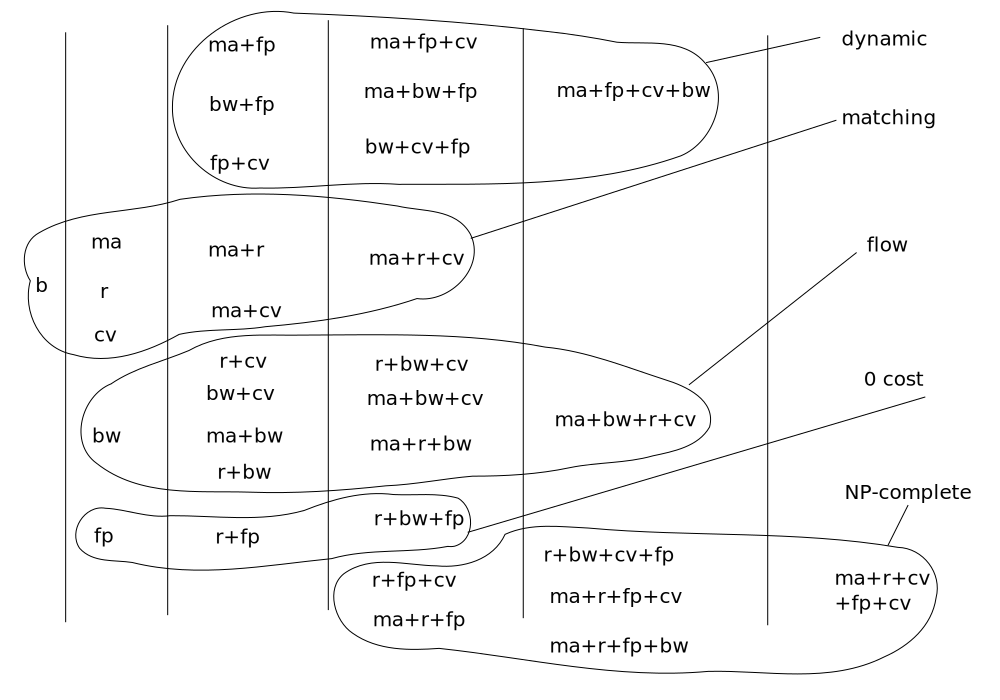
\includegraphics[width=\columnwidth]{figs/summary}
%\caption{\maciek{This figure is wrong in couple places, but I sent you an e-mail what should be redone.}Summary of results. As this paper only presented algorithms %(approaches indicated in the same
%color and pattern as in the previous figures) for the most
%difficult problems and, respectively, proved NP-hardness (indicated in black) of the simplest
%problems, several additional results are simple implications. In this figure,
%we always suggest the best (simplest and fastest) approach to solve a specific problem variant.}
%\label{fig:summary}
%\end{figure}


%\begin{figure}[t]
%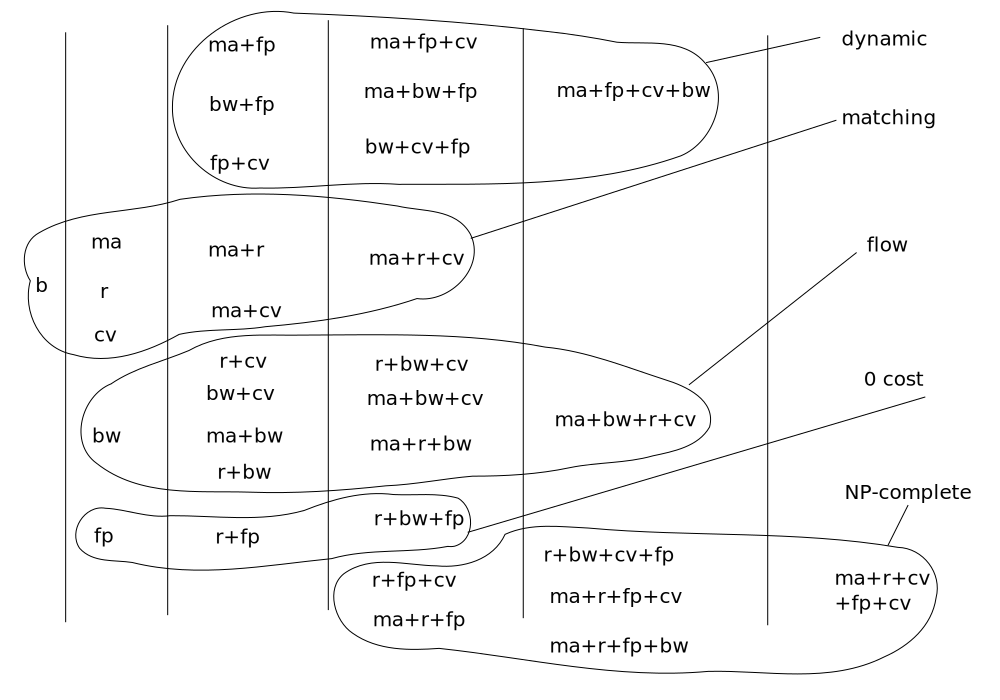
\includegraphics[width = \columnwidth]{figs/summary}
%\caption{Summary of results. As this paper only presented algorithms for the most
%difficult problems and, respectively, proved NP-hardness of the simplest
%problems, several additional results are simple implications (indicated by arrows).}
%\label{fig:summary}
%\end{figure}

%We believe that our paper opens several interesting directions for future research.
%In particular, it would be interesting to shed light on the possible approximation algorithms
%for our NP-hard problems.

\textbf{Acknowledgments.} We would like to thank 
Paolo Costa for many discussions. 
This research is in part supported by Polish National Science Centre grant DEC-2013/09/B/ST6/01538, the EU project Bigfoot FP7-ICT-317858,
as well as by the German BMBF Software Campus grant 01IS12056.

%%%%%%%%%%%%%%%%%%%%%%%%%%%%%%%%%%%%%
%\bibliographystyle{alpha}
{\footnotesize \renewcommand{\baselinestretch}{.9}
\bibliographystyle{abbrv}
\bibliography{references}
}

%\begin{appendix}


\end{document}
